\pdfoutput=1
\pdfminorversion=5
\pdfsuppresswarningpagegroup=1

\documentclass[preprint]{elsarticle}

\usepackage[utf8]{inputenc}

%packages
\usepackage[margin=1in]{geometry}

\usepackage[hyphens]{url}
\biboptions{sort&compress, square, comma}
\usepackage[breaklinks=true, linkcolor=blue, citecolor=blue, colorlinks=true]{hyperref}

\usepackage{graphicx}
\usepackage{caption}
\usepackage{subcaption}

%\captionsetup[algorithm]{labelformat=empty}

\usepackage{booktabs,multirow}
\usepackage[version=3]{mhchem} % Formula subscripts using \ce{}, e.g., \ce{H2SO4}
\usepackage{latexsym,amsmath,amssymb}

\usepackage{mathtools}
\usepackage{tablefootnote}

%better printing of numbers
\usepackage[T1]{fontenc}
\usepackage[english]{babel}
\usepackage{csquotes}
\usepackage{textcomp}

\usepackage{algorithm}
\usepackage[noend]{algpseudocode}
\makeatletter
\let\OldStatex\Statex
\renewcommand{\Statex}[1][3]{%
  \setlength\@tempdima{\algorithmicindent}%
  \OldStatex\hskip\dimexpr#1\@tempdima\relax}

\usepackage[binary-units]{siunitx}
\sisetup{group-separator={,},
     detect-all,
     binary-units,
     list-units = single,
     range-units = single,
     range-phrase = --, 
     per-mode = symbol-or-fraction,
     separate-uncertainty = true,
     multi-part-units = single,
     list-final-separator = {, and }
%    scientific-notation = fixed
}
\DeclareSIUnit\atm{atm}

\graphicspath{{./figures/}}

% Add [disable] option to quickly remove any
\usepackage[textsize=small,textwidth=2.25cm]{todonotes}

%custom commands
\newcommand{\NA}{---}
\newcommand{\centercell}[1]{\multicolumn{1}{c}{#1}}
\newcommand{\centermulti}[2]{\multicolumn{#2}{c}{#1}}
\newcommand{\head}[1]{\centercell{\bfseries#1}}
\newcommand{\headmulti}[2]{\centermulti{\bfseries#1}{#2}}

\newcommand{\argmax}{\operatornamewithlimits{argmax}}

\journal{Journal of Computational Physics}

\begin{document}

\begin{frontmatter}

\title{An investigation of GPU-based stiff chemical kinetics integration methods}

\author[uconn]{Nicholas~J.\ Curtis\corref{cor1}}
\ead{nicholas.curtis@uconn.edu}
\author[osu]{Kyle~E.\ Niemeyer}
\author[uconn]{Chih-Jen Sung}
%\ead{cjsung@engr.uconn.edu}

% addresses
\address[uconn]{Department of Mechanical Engineering\\
  University of Connecticut, Storrs, CT, 06269, USA}
\address[osu]{School of Mechanical, Industrial, and Manufacturing Engineering\\
  Oregon State University, Corvallis, OR 97331, USA}
  
\cortext[cor1]{Corresponding author}

\begin{abstract}
A fifth-order implicit Runge--Kutta method and two fourth-order exponential integration methods equipped with Krylov subspace approximations were implemented for the GPU and paired with the analytical chemical kinetic Jacobian software \texttt{pyJac}.
The performance of each was evaluated by integrating thermochemical state data sampled from stochastic partially stirred reactor simulations and compared with the commonly used CPU-based implicit integrator \texttt{CVODE}.
We estimate that the implicit Runge--Kutta method running on a single GPU is equivalent to \texttt{CVODE} running on \num{10} or more CPU cores (up to $\sim$\num{35}) for all but the most stiff case studied, where thread divergence significantly decreased performance.\todo[inline]{add numbers here?}
The exponential integration techniques performed more slowly for all cases.\todo[inline]{more slowly than what?}
Thread divergence and memory traffic were identified as the main limiters of GPU integrator performance, and techniques to mitigate these issues were discussed.
Use of an analytical Jacobian on the GPU was found to be critical for efficient integration, far surpassing the benefits of analytical Jacobian use on the CPU for identical problems.\todo[inline]{numbers here?}
Finally, future research directions were identified based on the current state-of-the-art of stiff chemical kinetics integration on the GPU.
\end{abstract}

\begin{keyword}
 Chemical kinetics \sep Stiff chemistry \sep Integration algorithms \sep GPU
\end{keyword}

\end{frontmatter}

\clearpage

%%%%%%%%%%%%%%%%%%%%%%%%%%%%%%%%%%%%%%%%%%%%
\section{Introduction}
\label{sec:Intro}
%%%%%%%%%%%%%%%%%%%%%%%%%%%%%%%%%%%%%%%%%%%%

The need for accurate chemical kinetic models in predictive reacting-flow simulations has driven the development of detailed oxidation models for hydrocarbon fuels relevant to transportation and energy generation applications.
At the same time, growing understanding of hydrocarbon oxidation processes resulted in orders of magnitude increases in model size and complexity.
For instance, a recently developed model for 2-methylalkanes, relevant for jet and diesel fuel surrogates, includes over \num{7000} species and \num{30000} reactions~\cite{Sarathy:2011kx} while a recent detailed gasoline surrogate mechanism contains over \num{1500} species and \num{6000} reactions~\cite{Mehl:2011jn}.\todo{some of this is pretty close to sentence in the pyJac paper; might want to revise}
Furthermore, kinetic models for large hydrocarbon fuels tend to exhibit high chemical stiffness that requires implicit integration algorithms for efficient solution.
The cost of these algorithms scales at best quadratically---and at worst cubically---with the number of species in a model~\cite{Lu:2009gh}.
Lu and Law~\cite{Lu:2009gh} extensively reviewed techniques to accelerate chemical kinetics integration.
In addition to the methods discussed in their work, significant effort has also been directed towards improvements of the integration algorithms.

Reactive-flow modeling codes commonly rely on high-order implicit integration techniques to solve the stiff governing equations posed by chemical kinetic models.
These methods require repeated evaluation and factorization of the chemical kinetic Jacobian matrix in order to solve the associated nonlinear algebraic equations through iterations of linear system solutions---the cost of which scales quadratically and cubically, respectively, with the number of species in a mechanism.
However, significant cost savings in the Jacobian evaluation can be realized by using an analytical formulation, rather than the typical evaluation via finite difference approximations.
This approach eliminates numerous chemical source term evaluations, and for a sparse Jacobian (e.g., formulated in terms of species concentrations) the cost of evaluation can drop to a linear dependence on the number of species in the mechanism~\cite{Lu:2009gh}.

In this work, our efforts to accelerate chemical kinetics focus on improving the integration strategy itself, via development of new algorithms and use of high-performance hardware accelerators such as graphics processing units (GPUs) and similar single-instruction multiple-data (SIMD) devices.
Central processing unit (CPU) clock speeds increased regularly over the past few decades---commonly known as Moore's Law---however, power consumption and heat dissipation issues slowed this trend recently.
While multicore parallelism somewhat increased CPU performance, recently SIMD processors gained popularity as a low cost, low power consumption, and massively parallel high-performance computing alternative.
GPUs were originally developed for graphics\slash video processing applications and consist of hundreds to thousands of separate processing cores\todo{is this the best term here?}, compared with the tens of cores found on typical CPUs.
The SIMD parallelism model differs from a traditional CPU-based multithreading model, with small per-core memory caches and acceleration resulting from executing the same instruction over multiple data.
Subsequently, using the SIMD parallelism model to accelerate chemical kinetics integration requires extra consideration.

This study used the NVIDIA CUDA framework~\cite{Buck:2008aa,NVIDIA:2015aa}, hence the following discussion will use CUDA terminology; however, the concepts within are widely applicable to SIMD processing.
The basic parallel function call on a GPU, termed a kernel, is broken up into a grid of thread blocks.
A GPU consists of a number of streaming multiprocessors (SMs), each of which is assigned one or more thread blocks in the grid.
The SMs further subdivide the blocks into groups of \num{32} threads called warps, which form the fundamental CUDA processing unit.
The resources available on a SM (memory, cores, registers, etc.) are split between the warps from all the assigned blocks.
The threads in a warp are executed in parallel on CUDA cores, with multiple warps typically being executed concurrently on a SM.
Thread divergence, a key performance concern for SIMD processing, occurs when the threads in a warp follow different execution paths, e.g., due to if\slash then branching.
In this case, the divergent execution paths must execute in serial, causing a slowdown.
Furthermore, as compared with a typical CPU, GPUs possess relatively small memory caches and few registers per SM.
These resources are further split between all the blocks\slash warps running on that SM.
Overuse of these resources can cause slow global memory accesses for data not stored locally in-cache or can even reduce the number of blocks assigned to each SM.
The performance tradeoffs of various CUDA execution patterns are quite involved and beyond the scope of this work, for more details we refer the interested reader to several works that discussed these topics in depth~\cite{Cruz:2011gc,Brodtkorb:2013hn,Niemeyer:2014hn}.
Instead, we will briefly highlight key considerations for CUDA-based chemical kinetic ODE integration.

The extent of thread-cooperation within a CUDA-based chemical kinetic ODE integration algorithm is a key point that shapes much of implementation.
Typically GPU accelerated chemical kinetic solvers follow either a ``per-thread'' pattern~\cite{Niemeyer:2011aa,Stone:2013aa,Niemeyer:2014aa}, in which each individual GPU thread solves a single set of chemical kinetic ODEs, or a ``per-block'' approach~\cite{Stone:2013aa,Sewerin20151375}, in which all the threads in a block cooperate to solve a single set of chemical kinetic ODEs.
The greatest potential benefit of a per-thread approach is that a much larger number of ODEs can theoretically be solved concurrently; typically the number of blocks that can be executed concurrently on each SM is around eight, whereas typical CUDA launch configurations in this work consist of 64 threads per block, or 512 sets of ODEs solved concurrently per SM.
Unfortunately, the larger amount of parallelism offered by a per-thread approach does not come without drawbacks.
For example, as the memory available per SM must now be split between many more sets of ODEs, a per-thread approach may encounter more cache-misses, resulting in expensive global memory loads.
The performance of a per-thread approach can also be greatly impacted by thread divergence, because different threads may follow different execution paths within the ODE integration algorithm itself~\cite{Stone:2013aa,Niemeyer:2014aa}.
For this reason, implicit integration algorithms, which typically have complex branching and evaluation paths, may suffer more from thread divergence when implemented on a per-thread basis than relatively simpler explicit integration techniques~\cite{Stone:2013aa}.
Thread divergence typically impacts integrators following a per-block strategy less severely, since the execution path of each thread is planned by design of the algorithm.
A per-block approach also offers significantly more local cache memory and available registers for solving a set of ODEs, and thus memory access speeds and cache size are less of a concern.
However, in our experience, optimizing use of these resources requires significant manual tuning, making it more difficult to generalize the developed algorithm between different chemical kinetic models (a key feature for potential non-academic applications).
Finally, past work has shown that in the best-case scenario---elimination of the majority of thread divergence by choice of identical initial conditions---the performance of a per-thread implicit integration algorithm greatly surpasses that of the per-block implementation of the same algorithm~\cite{Stone:2013aa}.
\todo[inline]{This paragraph had a lot of sentences in a row that started with a single word or phrase and a comma (However, For this reason, Conversely, Further, etc), which I tried to break up}

A number of studies in recent years explored the use of high-performance SIMD devices to accelerate (turbulent) reacting-flow simulations.
Spafford et al.~\cite{Spafford:2010aa} investigated the use of GPUs to accelerate a turbulent combustion direct numerical simulation code, demonstrating a sub-order of magnitude speedup in evaluating the species production rates on the GPU.
Shi et al.~\cite{Shi:2011aa} used a GPU to evaluate species rates and factorize the Jacobian for the integration of (single) independent kinetics systems, showing order-of-magnitude or greater speedups for large kinetic models.
Niemeyer et al.~\cite{Niemeyer:2011aa} implemented an explicit fourth-order Runge--Kutta integrator for the GPU, and found a speedup of nearly two orders of magnitude with a nonstiff hydrogen mechanism.
Shi et al.~\cite{Shi:2012aa} implemented a stabilized explicit solver for the GPU and paired it with a CPU-based implicit solver that handled integration of the most-stiff chemistry cells in a three-dimensional premixed diesel engine simulation, demonstrating an overall speedup of two to three times.
Le et al.~\cite{Le2013596} implemented GPU versions of two high-order shock-capturing reacting flow codes, and found a \numrange{30}{50}$\times$ speedup over the baseline.\todo{single CPU?}
Stone and Davis~\cite{Stone:2013aa} implemented the implicit VODE~\cite{Brown:1989vl} solver for the GPU and achieved an order of magnitude speed-up over the baseline CPU version.
Additionally, they showed that the implicit VODE algorithm exhibited significant thread divergence, as expected due to its complicated program flow (compared with an explicit integration scheme).
Furthermore, Stone and Davis~\cite{Stone:2013aa} showed that for $\sim$\num{e4} independent ODEs or more, a per-thread implementation outperformed a per-block version of the same algorithm; the per-block implementation reached its maximum speedup for a smaller number of ODEs ($\sim$\num{e3}).
Niemeyer and Sung~\cite{Niemeyer:2014aa} demonstrated an order-of-magnitude speedup for a GPU implementation of a stabilized explicit second-order Runge--Kutta--Chebyshev algorithm over a multicore CPU implementation of VODE for moderately stiff chemical kinetics.
They also investigated levels of thread divergence due to differing integrator time-step sizes, and found it negatively impacts overall performance for dissimilar ODE initial conditions in a thread-block.
Sewerin and Rigopoulos~\cite{Sewerin20151375} implemented a three-stage\slash fifth-order implicit Runge--Kutta method~\cite{wanner1991solving} on a one-block per ODE basis on GPU, and found a \num{1.8}$\times$ slowdown at best compared with the same on a single eight-core CPU.

While increasing numbers of studies have explored GPU-based chemical kinetics integration, there remains a clear need to find or develop integration algorithms simultaneously suited for the SIMD parallelism of GPUs (along with similar hardware accelerators) and capable of handling stiffness.
In this work we will investigate GPU implementations of several explicit and implicit integration techniques, as compared to their CPU counterparts and the baseline CPU \texttt{CVODE}~\cite{Hindmarsh:2005hg} algorithm.
Several previous works~\cite{Perini20141180,McNenly2015581} suggested so-called matrix-free methods---which do not require direct factorization of the Jacobian, but instead use an iterative process to approximate the action of the factorized Jacobian on a vector---as potential improvements to the expensive linear-system solver required in standard implicit methods.
Furthermore, Hochbruck and Lubich~\cite{Hochbruck:1997} demonstrated that the action of the matrix exponential on a vector obtained using Krylov subspace approximation converges faster than corresponding Krylov methods for the solution of linear equations.
Others previously explored these so-called explicit exponential methods for applications in stiff chemical systems~\cite{Bisetti:2012jw,falati2011integration} and found them stable for time-step sizes greatly exceeding the stability bound.
In addition, their explicit nature makes them potentially better suited for SIMD acceleration due to an expected reduction of thread divergence (for a per-thread implementation) compared with implicit methods.
Finally, the three-stage\slash fifth-order implicit Runge--Kutta algorithm~\cite{wanner1991solving} investigated by Sewerin and Rigopoulos~\cite{Sewerin20151375} will be studied to determine the impact of increasing chemical stiffness on the algorithm and the performance benefits of using an analytical Jacobian matrix, such as that developed by Niemeyer et al.~\cite{niemeyer_2016_51139,Niemeyer:2015ws,Niemeyer:2016aa}.

The rest of the paper is structured as follows.
Section~\ref{S:method} lays out the methods and implementation details of the algorithms used here.
Subsequently, Sec.~\ref{S:results} presents and discusses the performance of the algorithms run using a database of partially stirred reactor thermochemical states, with particular focus on the effects of thread divergence and the potential impacts of current state-of-the-art GPU-accelerated chemical kinetic evaluation for large-scale reacting flow simulations.
Finally, Sec.~\ref{S:conclusions} uses the results of this work to identify the most promising future directions for GPU\slash SIMD accelerated chemical kinetic integration.

%%%%%%%%%%%%%%%%%%%%%%%%%%%%%%%%%%%%%%%%%%%%
\section{Methodology}
\label{S:method}
%%%%%%%%%%%%%%%%%%%%%%%%%%%%%%%%%%%%%%%%%%%%

In this section, we discuss details of the algorithms implemented for the GPU along with third-party software used.
The generation of testing conditions will be discussed briefly, and the developed solvers will be validated.

%%%%%%%%%%%%%%%%%%%%%%%%%%%%%%%%%%%%%%%%%%%%
\subsection{Integration techniques}

We investigated GPU implementations of three integration methods in this work, comparing them against equivalent CPU versions and a CPU-only implicit algorithm.
While we describe important details or changes here, full descriptions of all algorithms may be found in the cited sources.
The \texttt{pyJac} software~\cite{niemeyer_2016_51139,Niemeyer:2015ws,Niemeyer:2016aa} provided both chemical source term and analytical Jacobian subroutines for CPU- and GPU-based algorithms.
We evaluated the relative performance impact of using a finite-difference Jacobian matrix (as compared with an analytical Jacobian) for both platforms with a first-order finite difference method based on that of \texttt{CVODE}~\cite{Hindmarsh:2005hg}.
The chemical source terms used by the finite-difference Jacobian were provided by \texttt{pyJac} in all cases.
We direct readers to our previous work~\cite{Niemeyer:2015ws,Niemeyer:2016aa} for validation and performance assessments of \texttt{pyJac} itself.

First, the \texttt{CVODE} solver~\cite{Hindmarsh:2005hg} provided the baseline performance of a typical CPU-based (maximum of fifth-order) implicit integration technique.\todo{need to cite the specific version here}
In addition, we implemented CPU versions of the methods under investigation for direct comparison to the high-order implicit technique.
These include the three-stage\slash fifth-order implicit Runge--Kutta algorithm~\cite{wanner1991solving} (\texttt{Radau-IIA}), the fourth-order exponential Rosenbrock-like method of Hochbruck et al.~\cite{Hochbruck:1998} (\texttt{exp4}), and the newer fourth-order exponential Rosenbrock method~\cite{Hockbruck:2009} (\texttt{exprb43}).
For the exponential methods, we used the method of rational approximants~\cite{gallopoulos:1992} paired with the Carath\'edothy--Fej\'er method~\cite{trefethen:2006}\todo{cite Kyle's code} to approximate the action of the matrix exponential on a vector, as suggested by Bisetti~\cite{Bisetti:2012jw}.
This technique relied on the external \texttt{FFTW3} library~\cite{frigo2005design}.\todo{need to cite specific FFTW3 version too}
However, unlike the approach of Bisetti~\cite{Bisetti:2012jw}, we developed a custom routine based on the algorithm presented by Stewart~\cite{stewart:1998} to perform LU decomposition of the Hessenberg matrix resulting from the Arnoldi iteration.
Convergence of the Arnoldi iteration algorithm was computed using the second term of the exponential matrix\slash vector product infinite series, as suggested in several works~\cite{Bisetti:2012jw,saad:1992}.
The exponential integrators used a rational approximant type of $\left(10,10\right)$ as suggested by Bisetti~\cite{Bisetti:2012jw}.
To ensure high performance of CPU-based methods, the Intel \texttt{MKL} library version 11.3.2 handled linear algebra (i.e., BLAS/LAPACK) operations.
Next, we implemented GPU versions of the \texttt{Radau-IIA}, \texttt{exp4}, and \texttt{exprb43} methods.
These follow the same descriptions as the CPU versions, but require specialized implementations of several BLAS and LAPACK methods, mostly related to LU factorization of the Jacobian or Hessenberg matrices.
All GPU routines were developed using the NVIDIA CUDA framework~\cite{Buck:2008aa,NVIDIA:2015aa}.
The \texttt{Radau-IIA} solver as developed by Hairer and Wanner~\cite{wanner1991solving} contains an adaptive time-stepping technique, the exponential methods used a standard adaptive time-stepping technique~\cite{wanner1991solving}; adaptive time-stepping was handled internally by the \texttt{CVODE} solver.\todo{not quite sure what's going on with this sentence, but it's definitely confusing}
Finally, the adaptive time stepping procedures of all integrators used absolute and relative tolerances of \SI{e-10} and \SI{e-6}, respectively, throughout the work.

%%%%%%%%%%%%%%%%%%%%%%%%%%%%%%%%%%%%%%%%%%%%
\subsection{Testing conditions}
\label{S:pasr_conditions}

In order to measure the performance of the integrators for realistic conditions, a database of thermochemical states covering a wide range of temperatures and species mass fractions was generated using a previously developed constant-pressure stochastic partially stirred reactor (PaSR) code~\cite{Niemeyer:2016aa,niemeyer_2016_51139}.
We selected two chemical kinetic models to span the range of model sizes typically used in high-fidelity simulations: the \ce{H2}\slash\ce{CO} model of Burke et al.~\cite{Burke:2011fh} with 13 species and 27 reactions, and the GRI-Mech 3.0 model with 53 species and 325 reactions~\cite{smith_gri-mech_30}.
The PaSR simulations were performed at the conditions listed in Table~\ref{T:pasr_parameters} for 10 residence times to reach a statistical steady state; Niemeyer et al.~\cite{Niemeyer:2016aa} describe the PaSR simulation process in greater detail, which follows approaches used by others~\cite{Chen:1997ta,Pope:1997wu,Ren:2014cd}.
The PaSR particles were initialized using the equilibrium state, and gradually move away from equilibrium conditions due to mixing, inflow, and outflow.
In order to reduce the influence of the equilibrium condition on the solution runtime trends for small numbers of ODEs, the first \num{1000} datapoints (corresponding to a single $\tau_\text{pair}$ time interval) were removed from each database.
At this point in the simulation, $\sim\SI{80}{\percent}$ of the particles were at or near an equilibrium state, and by the \num{5000}th datapoint only $\sim\SI{20}{\percent}$ of the particles were near equilibrium.\todo{Reworded this a bit, check it out. Also might be informative to give the total number of datapoints to give some context}

\begin{table}[htb]
\centering
\begin{tabular}{@{}l l l @{}}
\toprule
Parameter & \ce{H2}\slash air & \ce{CH4}\slash air \\
\midrule
$\phi$ & \multicolumn{2}{c}{1} \\
$T_{\text{in}}$ & \multicolumn{2}{c}{\SIlist{400;600;800}{\kelvin}} \\
$p$ & \multicolumn{2}{c}{\SIlist{1;10;25}{\atm}} \\
$N_p$ & \multicolumn{2}{c}{100} \\
$\tau_{\text{res}}$ & \SI{10}{\milli\second} & \SI{5}{\milli\second} \\
$\tau_{\text{mix}}$ & \SI{1}{\milli\second} & \SI{1}{\milli\second} \\
$\tau_{\text{pair}}$ & \SI{1}{\milli\second} & \SI{1}{\milli\second} \\
\bottomrule
\end{tabular}
\caption{
PaSR parameters used for hydrogen\slash air and methane\slash air premixed combustion cases, where $\phi$ indicates equivalence ratio, $T_{\text{in}}$ is the temperature of the inflowing particles, $p$ is the pressure, $N_p$ is the number of particles, $\tau_{\text{res}}$ is the residence time, $\tau_{\text{mix}}$ is the mixing time, and $\tau_{\text{pair}}$ is the pairing time.
}
\label{T:pasr_parameters}
\end{table}

%%%%%%%%%%%%%%%%%%%%%%%%%%%%%%%%%%%%%%%%%%%%
% \subsection{Shared memory caching}
% \label{S:smem_present}
% 
% A unique memory-access pattern is one aspect of the GPU platform particularly important to high-performance algorithms; each streaming multiprocessor can access only a small amount of fast cache memory (typically \SI{64}{\kilo\byte}) and \SI{32}{\bit} registers (typically \SIrange{32}{64}{\kilo\byte}).
% All other memory is stored globally on the device, with comparatively high latencies.
% Thus, it is critical to properly use cache memory to achieve maximum performance on GPUs.
% When formulated on a per-block basis, GPU-based integration algorithms typically use this memory to store commonly used values such as the current state vector and  chemical Jacobian.
% However, on a per-thread basis, the best use of this memory is less clear; this section proposes one approach for efficient use of this fast memory.
% 
% Using fast memory on a per-thread basis poses a challenge: it must be split between all threads in the blocks resident on a streaming multiprocessor.
% This fast memory is further split into an L1 cache and shared memory available for interthread communication within a block.
% Most versions of the CUDA compute standards allow the user to specify the relative allocation of the L1 cache and shared memory pool.
% In our preliminary studies, a larger L1 cache proved the superior choice for our per-thread approach; the inherent increased memory traffic quickly overwhelms the small cache memory, resulting in slower global memory accesses.
% However, this left $\sim$\SI{16}{\kilo\byte} of the cache memory as shared memory, with only around two to four double-precision variables available per thread.
% This small amount of available memory is challenging to use in the integration algorithm itself; however, evaluation of the chemical source terms and analytical Jacobian present opportunities for using the shared memory.
% 
% \begin{algorithm}[htb]
% \caption{\textbf{Algorithm:} A procedure for memory caching during evaluation of reaction rates.\label{A:shared_mem_caching}}
% \begin{algorithmic}[0]
%   \State {Initialize the cached species concentration set $C = \varnothing$}
%   \State {Let maximum set size be $C_{\max}$}
%   \For {reaction $r_i$ of reactions $R$}
%     \State Let $S_i$ be the set of participating species in $r_i$
%     \State Let $P_{i,j}$ be the number of consecutive reactions starting from $r_{i + 1}$ in which each species $s_{i,j} \in S_i$ participates
%     \State For each species $c_j \in C$ let $L_j$ be the number of reactions since $c_j$ directly participated in a reaction
%     \State Priority sort the species $s_{i,j}$ in $S_{i}$ in descending order by priority $P_{i,j}$ and store in $S_{i}^{\prime}$
%     \For {$s_{i,j}$ in $S_{i}^{\prime}$}
%       \If{$|C| < C_{\max}$}
% 		\State Remove $s_{i,j}$ from $S_{i}^{\prime}$ and add to $C$
%       \ElsIf{$\max_l \left( L_l \right) \geq 2$ and $P_{i,j}$ > 1}
% 	  \State Let $k = \argmax_l \left(L_l \right)$
% 	  \State Remove $s_{i,j}$ from $S_{i}^{\prime}$ and replace $c_k$ in $C$ with $s_{i,j}$
%       \EndIf
%     \EndFor
%     \For {$s_{i,j}$ in $S_{i}^{\prime}$}
%       \If{$| S_{i}^{\prime} | > 0$ and $ |C| < C_{\max}$}
% 		\State Remove $s_{i,j}$ from $S_{i}^{\prime}$ and add to $C$
%       \EndIf
%     \EndFor
%     \State Load into shared memory all values in $C$ not already stored there.
%     \State Write code for evaluation of $i$th reaction rate using values in $C$ in place of global memory loads where possible.
%   \EndFor
% \end{algorithmic}
% \end{algorithm}
% 
% The presented~\hyperref[A:shared_mem_caching]{algorithm} describes a strategy to use this available shared memory to store commonly used species concentrations during evaluation of the reaction rates.
% Similar algorithms were developed for the species net production rates and Jacobian evaluation routines, using frequently updated species net production rates and frequently used reaction rates\slash species concentrations as the cached variables, respectively.
% As this algorithm runs during generation of the source code for the various subroutines, it introduces no computational or memory overhead related to determining the caching structure during runtime.
% Although this represents a relatively simple improvement, its use can achieve reasonable performance benefits, as will be seen in Sec.~\ref{S:smem}.

\subsection{Solver validation}

\begin{figure}[htb]
  \centering
  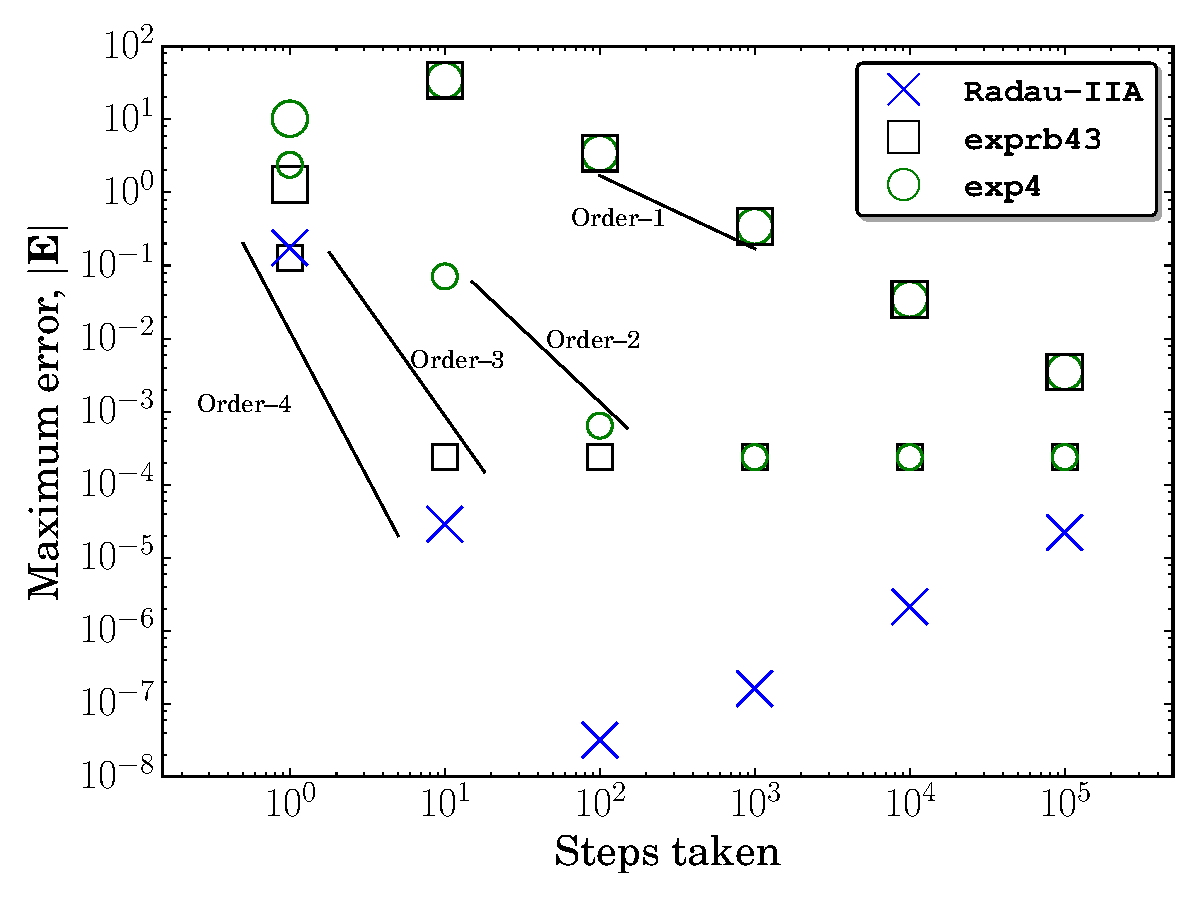
\includegraphics[width=0.7\linewidth]{c_nco_nosmem_error.pdf}
  \caption{Maximum error of the various CPU solvers as a function of global integrator time-step size $\delta t$.}
  \label{F:convergence}
  \todo[inline]{any additional points at larger time step size, to help indicate the order for Radau? or, can you indicate an order line based on the last two points? Without that, this figure seems incomplete}
\end{figure}

To investigate the correctness of the developed solvers, the first \num{10000} conditions in the \ce{H2}\slash\ce{CO} database were integrated by each solver for \SI{e-6}{\second}.
The error for condition $i$ was then determined using the weighted root-mean-square error
\begin{equation}
 E_i(t) = \left\lVert\frac{y_i(t) - \hat{y}_i(t)}{\text{atol} + \hat{y}_i(t) \cdot \text{rtol}}\right\rVert_2 \;,
\end{equation}
where the $y_i(t)$ is the solution obtained from the various solvers, and $\hat{y}_i(t)$ is the ``true'' solution obtained via \texttt{CVODE} using a global time-step of $\delta t = \SI{e-10}{\second}$ and absolute\slash relative tolerances of \num{e-20} and \num{e-15} respectively.
The maximum error over all conditions
\begin{equation}
 \left\lvert\textbf{E}\right\rvert = \max_{i= 1, \dots, \num{10000}}\{E_i(t)\}
\end{equation}
was then used to measure convergence.\todo{not sure what you mean by convergence here}
The solvers used the same tolerances as for the performance testing (absolute and relative tolerances of \num{e-10} and \num{e-6}, respectively).
Adaptive time-stepping was used in all cases, and Krylov subspace approximation was enabled for the exponential integrators thus evaluating the accuracy of the solvers, in identical form as used for performance testing.\todo{I think this sentence is incomplete, or needs editing for clarity}
The global integrator time-step was varied from \SI{e-6}{\second} to \SI{e-11}{\second} to examine convergence to the true solution.

Figure~\ref{F:convergence} shows the convergence plot for the CPU solvers.
The error of the \texttt{Radau-IIA} integrator is far below the specified integration tolerances (which normally select a time-step size to achieve $\left\lvert\textbf{E}\right\rvert \leq 1$) for all cases.
The exponential solvers exhibit much larger levels of error for the larger global time-step, with $\left\lvert\textbf{E}\right\rvert \sim \mathcal{O}(1)$ for the largest global time-step.
As the time-step size is decreased, two factors affect the overall error.
First, the internal integration time-step size was not held constant but instead allowed to vary adaptively, hence this is only a ``true'' convergence plot for the smaller time-step sizes where the global integrator step size is smaller than any taken by the adaptive scheme.
In conjunction, the convergence of the Arnoldi algorithm is affected by the internal integration time-step size (the matrix exponentials and error estimates are scaled by the internal step size).
To study the effect of the Arnoldi algorithm on the overall error, Fig.~\ref{F:convergence} also presents the convergence of the exponential integrators with the Krylov approximation error reduced far below the error of the overall method.
Practically, this is accomplished by detecting when the $n$th Krylov subspace vector approaches zero, a condition known as the ``happy breakdown'' in literature~\cite{datta2010numerical}.
In this limit, the approximate exponential matrix\slash vector product approaches the exact value and thus the error induced by the Krylov approximation is negligible.
In Fig.~\ref{F:convergence} is it seen that with the approximate Krylov subspace, the exponential methods achieve only first-order convergence to the true solution, but with the ``exact'' Krylov subspace both methods approach second-order convergence.
Although both methods are nominally fourth order, the combination of chemical stiffness and adaptive time-stepping reduces the apparent convergence to order two.
Furthermore, the error of Krylov subspace approximation dominates the error measurement $\lvert\textbf{E}\rvert$.
From Fig.~\ref{F:convergence} we may conclude that all solvers produce reasonably accurate solutions as compared to \texttt{CVODE}.
Additionally, although not shown, the results for the GPU solvers are nearly identical.


%%%%%%%%%%%%%%%%%%%%%%%%%%%%%%%%%%%%%%%%%%%%
\section{Results and discussion}
\label{S:results}
%%%%%%%%%%%%%%%%%%%%%%%%%%%%%%%%%%%%%%%%%%%%

We studied the performance of the integrators by testing each on the PaSR conditions described in Sec.~\ref{S:pasr_conditions} for two different global integration time-step sizes: $\delta t = \SI{e-6}{\s}$ and $\delta t = \SI{e-4}{\s}$, representative of those used in large eddy and Reynolds-averaged Navier--Stokes simulations, respectively.\todo{may be good to add citations for these numbers, so that they don't look like we pulled them out of midair}
Furthermore, the use of a larger global time step induces additional stiffness for a given model and enables evaluation of integrator performance at varying stiffness levels.
Runtimes are reported as the average over five runs, where each run started from the same set of PaSR conditions.
All CPU integrators were compiled using \texttt{gcc 4.8.5} (with the compiler options ``\texttt{-O3 -funroll-loops -mtune=native}''), and were executed in parallel via OpenMP on four ten-core \SI{2.2}{\giga\hertz} Intel Xeon E5-4640 v2 CPUs with \SI{20}{\mega\byte} of L3 cache memory.
OpenMP was used to parallelize on a per-condition basis; i.e., each individual OpenMP thread was responsible for integrating a single set of chemical kinetic ODEs, rather than cooperating with other OpenMP threads to solve the same.
A six-core \SI{2.67}{\giga\hertz} Intel Xeon X5650 was used as the host CPU for the GPU integrators, which were compiled using \texttt{nvcc 7.5.17} (with compiler options ``\texttt{-arch=sm\_20 -O3 -maxrregcount 63 -{}-ftz=false -{}-prec-div=true -{}-prec-sqrt=true -{}-fmad=false}'') and run on a single NVIDIA Tesla C2075 with \SI{6}{\giga\byte} of global memory.
Reported runtimes for the GPU-based algorithms include time needed for CPU--GPU data transfer before and after each global time step; in addition, the function \texttt{cudaSetDevice()} was used to initialize the GPU before timing to avoid any device initialization delay.
The open-source \texttt{pyJac} software~\cite{niemeyer_2016_51139,Niemeyer:2015ws,Niemeyer:2016aa} produced CPU and GPU custom source-code functions for the chemical source terms and analytical Jacobian matrix evaluation.
Finally, the L1\slash shared-memory cache was set to prefer a larger L1 cache using the \texttt{cudaDeviceSetCacheConfig()} function.

\subsection{Performance}

The integrator runtimes presented in this section were normalized by the number of ODEs solved for all cases.
The reasoning behind this presentation is two-fold.
First, saturation of the available computational resources becomes visually apparent (transition from a nearly linear decrease to a flat trend), and second, it allows certain other performance trends (e.g., the effects of thread divergence) to be easily highlighted.
The presentation of the performance data in raw form has been made available in \ref{S:raw} for completeness.

\begin{figure}[htb]
  \centering
  \begin{subfigure}{0.49\textwidth}
      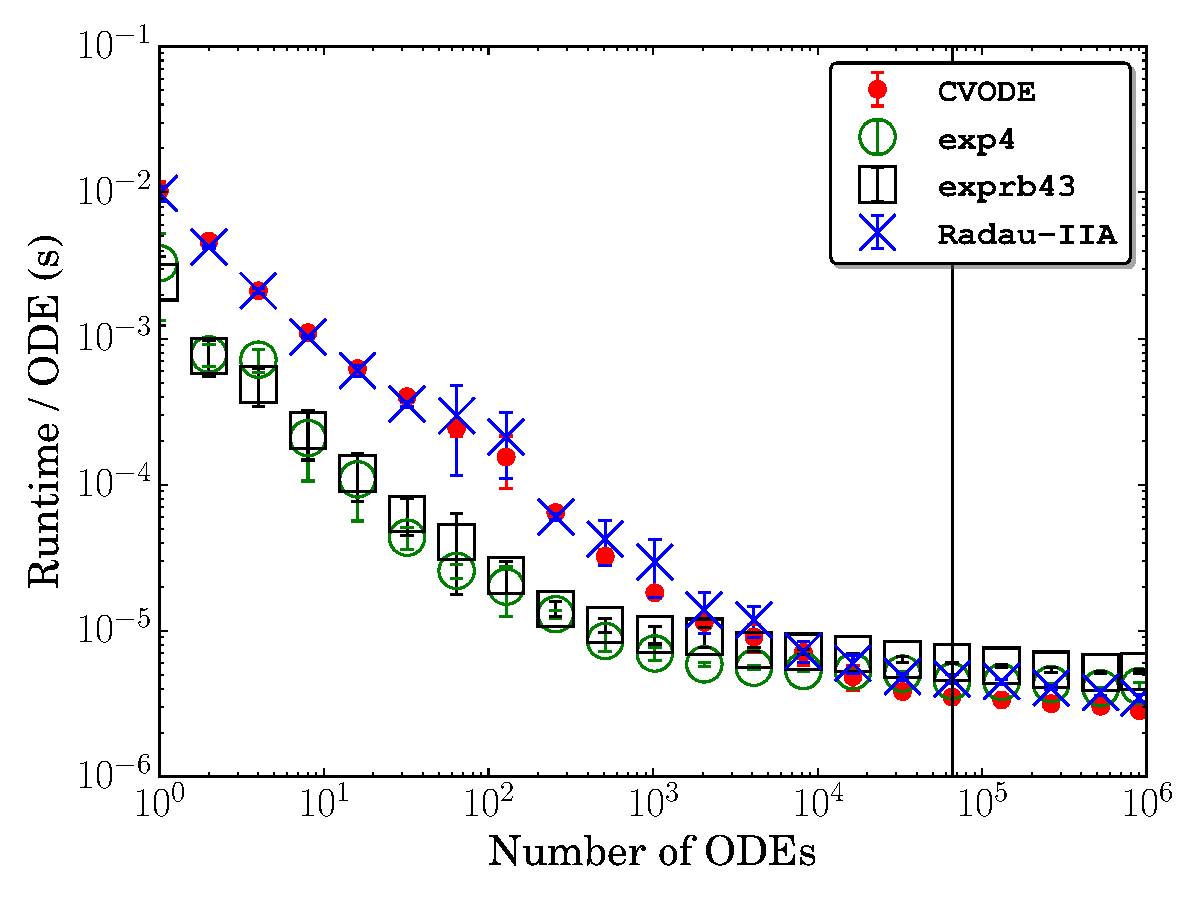
\includegraphics[width=\linewidth]{H2_1e-06_cpu.pdf}
      \caption{CPU performance for $\delta t = \SI{e-6}{\second}$}
      \label{F:h2_cpu_perf_small}
  \end{subfigure}
  %\hfill
  \begin{subfigure}{0.49\textwidth}
      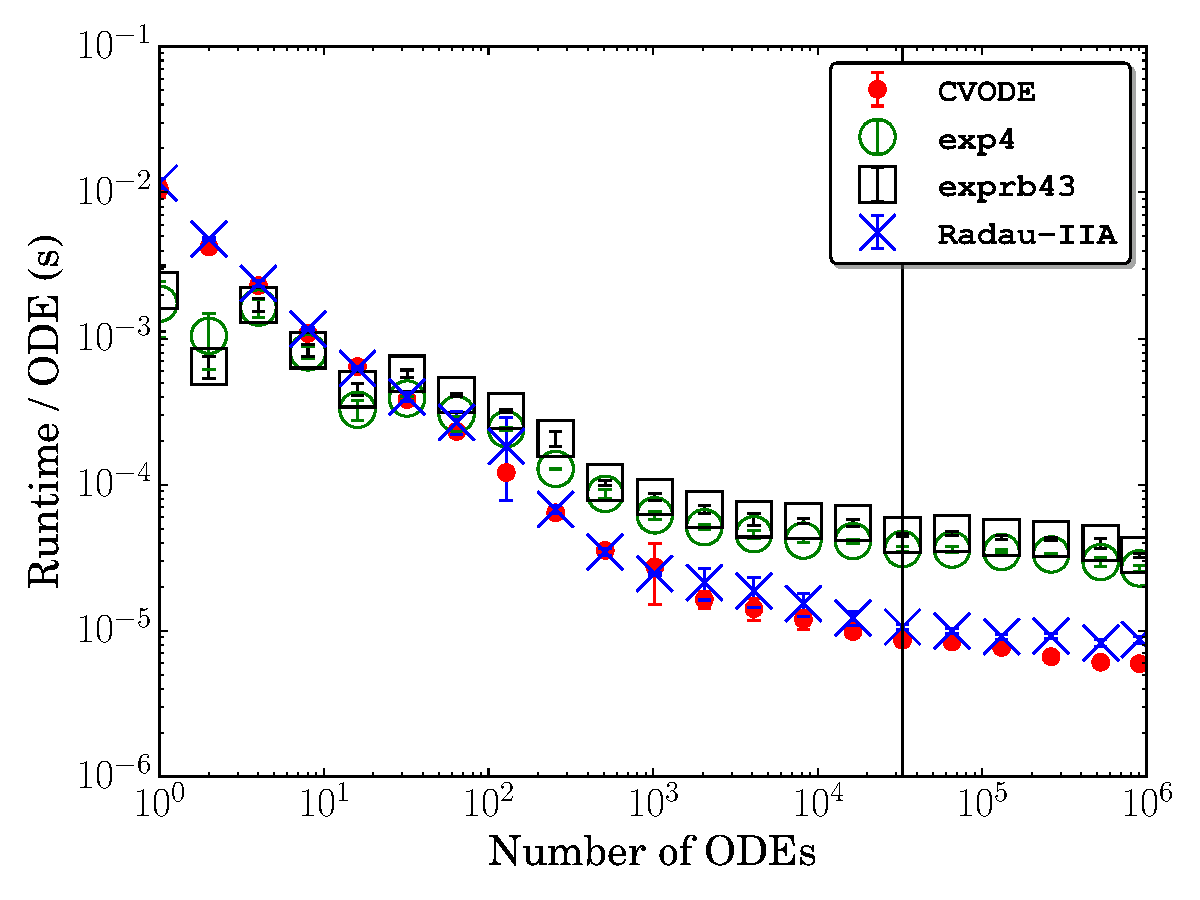
\includegraphics[width=\linewidth]{H2_1e-04_cpu.pdf}
      \caption{CPU performance for $\delta t = \SI{e-4}{\second}$}
      \label{F:h2_cpu_perf_large}
  \end{subfigure}\\
  \begin{subfigure}{0.49\textwidth}
      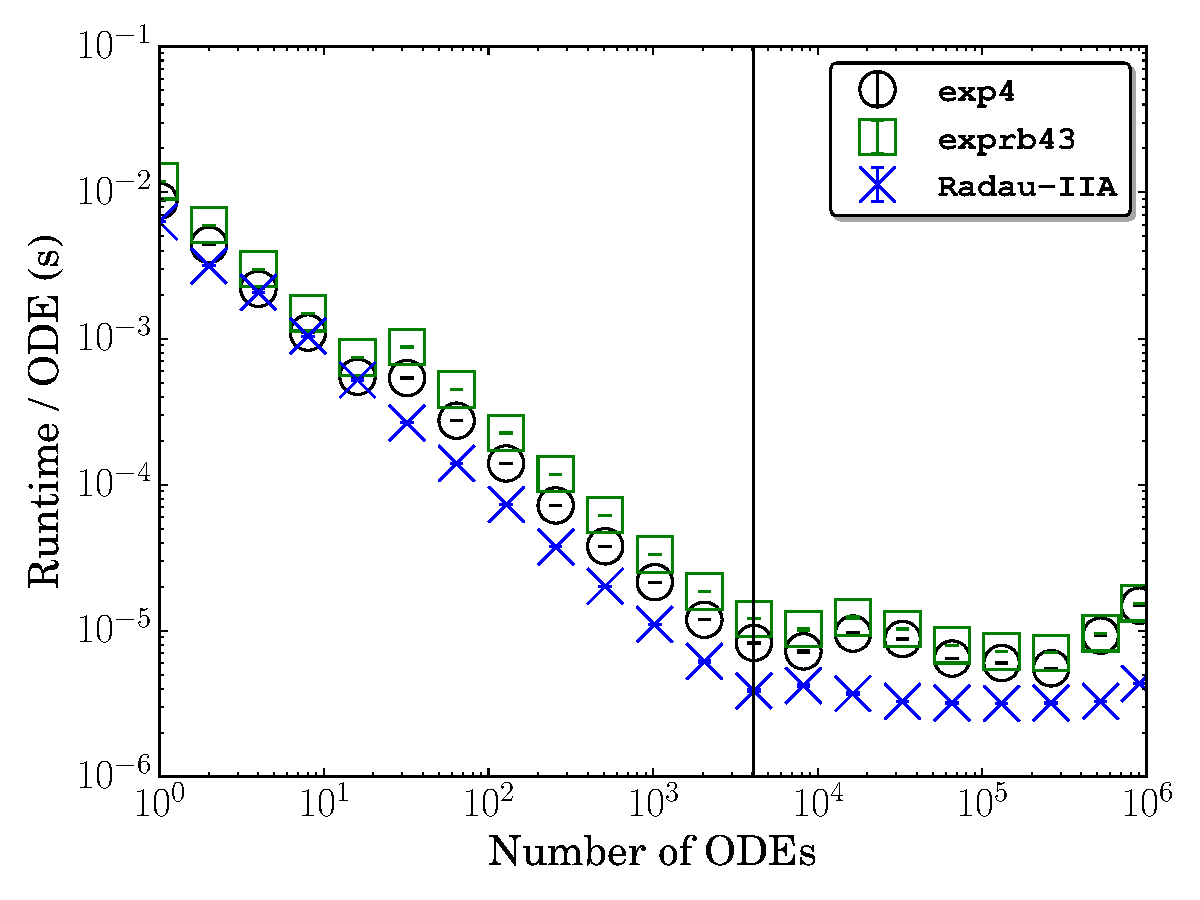
\includegraphics[width=\linewidth]{H2_1e-06_gpu.pdf}
      \caption{GPU performance results for $\delta t = \SI{e-6}{\second}$}
      \label{F:h2_gpu_perf_small}
  \end{subfigure}
  %\hfill
  \begin{subfigure}{0.49\textwidth}
      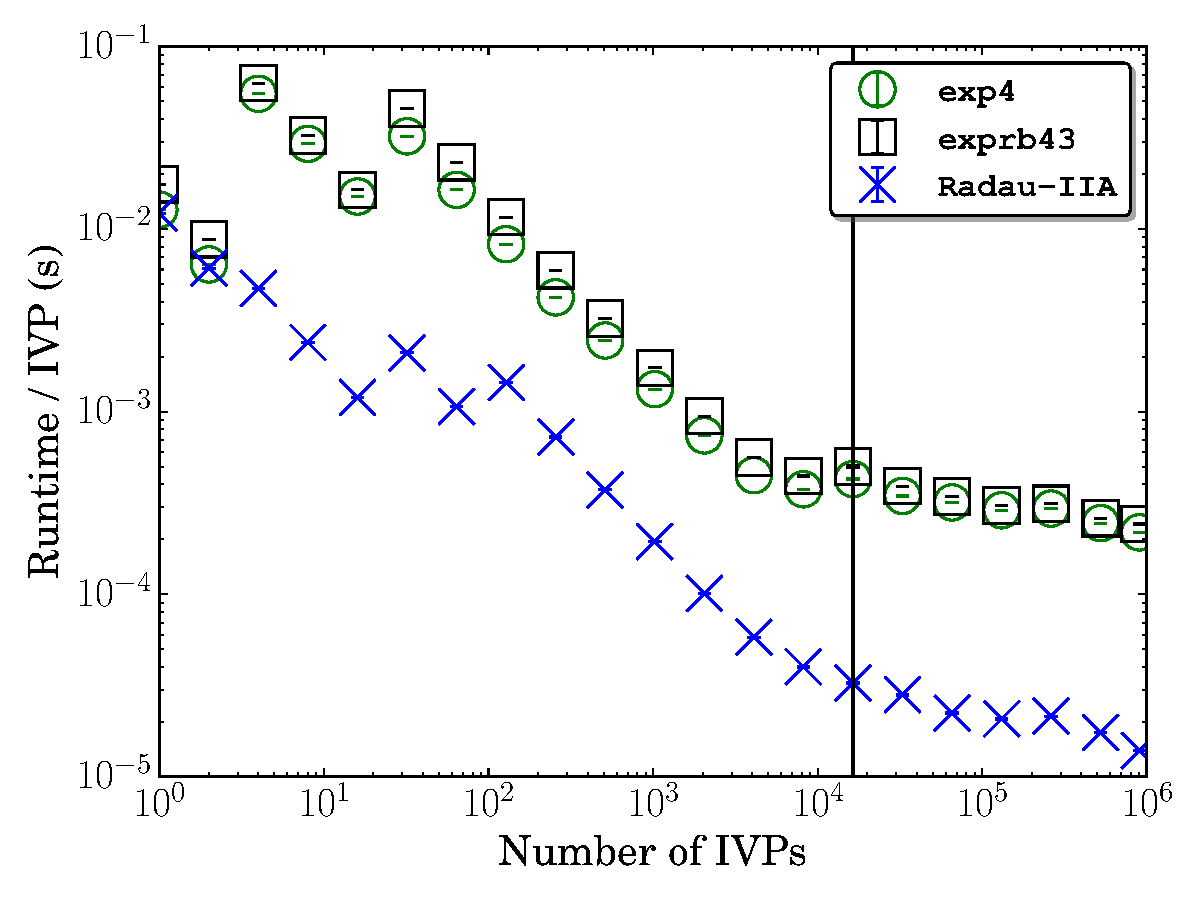
\includegraphics[width=\linewidth]{H2_1e-04_gpu.pdf}
      \caption{GPU performance results for $\delta t = \SI{e-4}{\second}$}
      \label{F:h2_gpu_perf_large}
  \end{subfigure}
  \caption{Average runtimes of the integrators on the CPU and GPU, scaled by the number of ODEs, for the \ce{H2}\slash\ce{CO} model at two different global time-step sizes.
  Estimation of where the runtime per ODE reaches a constant value (based on the results for \texttt{CVODE}\slash\texttt{Radau-IIA} for the CPU\slash GPU respectively) is marked in with a vertical line for all cases.
  Error bars indicate standard deviation.}
  \label{F:H2_perf}
\end{figure}

Figure~\ref{F:H2_perf} shows the runtimes of the CPU and GPU integrators for the \ce{H2}\slash\ce{CO} model.
In Fig.~\ref{F:h2_cpu_perf_small} the runtimes per ODE for the CPU integrators with a global time-step of $\delta t= \SI{e-6}{\second}$ decrease approximately linearly with the number of ODEs for small numbers of initial conditions (shown here on a log-log plot).
For small numbers of ODEs, the exponential integrators outperform the implicit integration techniques due to the modest stiffness of the \ce{H2}\slash\ce{CO} model; even with many near-equilibrium states removed from the beginning of the PaSR database, the model is not particularly stiff for this small time-step.
Larger numbers of ODEs begin to saturate the CPU resources, and the runtime per ODE levels off to a more constant value.
Eventually, relatively more stiff conditions are encountered and the performance of the implicit integration techniques catches up and then surpasses that of the exponential integrators; \texttt{CVODE} is the most efficient solver on the CPU when solving more than \num{e4} ODEs; however, the other solvers are of relatively similar efficiency in this case.\todo{replace the last bit of this sentence with numbers}{}
Fig.~\ref{F:h2_gpu_perf_small} shows the performance of the GPU integrators for the smaller global time-step, which exhibit similar trends as the CPU solvers: a linearly decreasing solution cost that reaches a roughly constant value between \numrange{e3}{e4} ODEs.
Unlike for the CPU solvers, the GPU-based \texttt{Radau-IIA} performs faster than the exponential solvers for all numbers of ODEs.
As will be seen in Sec.~\ref{S:divergence}, both solver classes experience minimal thread divergence due to differing internal integration time-step size in this case.
Therefore, we conclude that this difference results from thread divergence in the Arnoldi iteration---caused by varying Krylov subspace sizes between threads---for the exponential algorithms.

Figures~\ref{F:h2_cpu_perf_large} and \ref{F:h2_gpu_perf_large} show the performance of the integration algorithms on both platforms for the \ce{H2}\slash\ce{CO} model with the larger global time-step ($\delta t=\SI{e-4}{\second}$).
The performances of the CPU integration algorithms show similar trends to those of the smaller time-step case: decreasing cost per ODE before reaching a more constant performance for higher numbers of ODEs.
The larger time-step induces additional stiffness, and the implicit solvers are more efficient for most numbers of ODEs; \texttt{CVODE} is again the most efficient CPU solver.
Fig.~\ref{F:h2_gpu_perf_large} shows the performance of the GPU solvers for the larger time-step.
The exponential solvers exhibit significant spikes in computational cost for 4 and 32 ODE systems, with the latter mimicked somewhat by the implicit \texttt{Radau-IIA} solver.
The CPU solvers also show a performance decrease at four ODEs, indicating chemical stiffness as the primary cause.\todo{I don't actually see that at 4 ODEs, although I see a gap between CVODE\slash Radau and the exponential solvers at 2}
On the other hand, at 32 ODEs the CPU exponential solvers exhibit little-to-no performance decrease, while the GPU-based \texttt{Radau-IIA} also shows a decrease in performance at the same point---a trend completely absent in the CPU version.
These factors indicate that thread divergence is also playing a key role in the performance trend here, and will be investigated further in Sec.~\ref{S:divergence}.
As in the smaller global time-step case, the \texttt{Radua-IIA} solver is the most efficient GPU algorithm in all cases.

\begin{figure}[htb]
  \centering
  \begin{subfigure}{0.49\textwidth}
      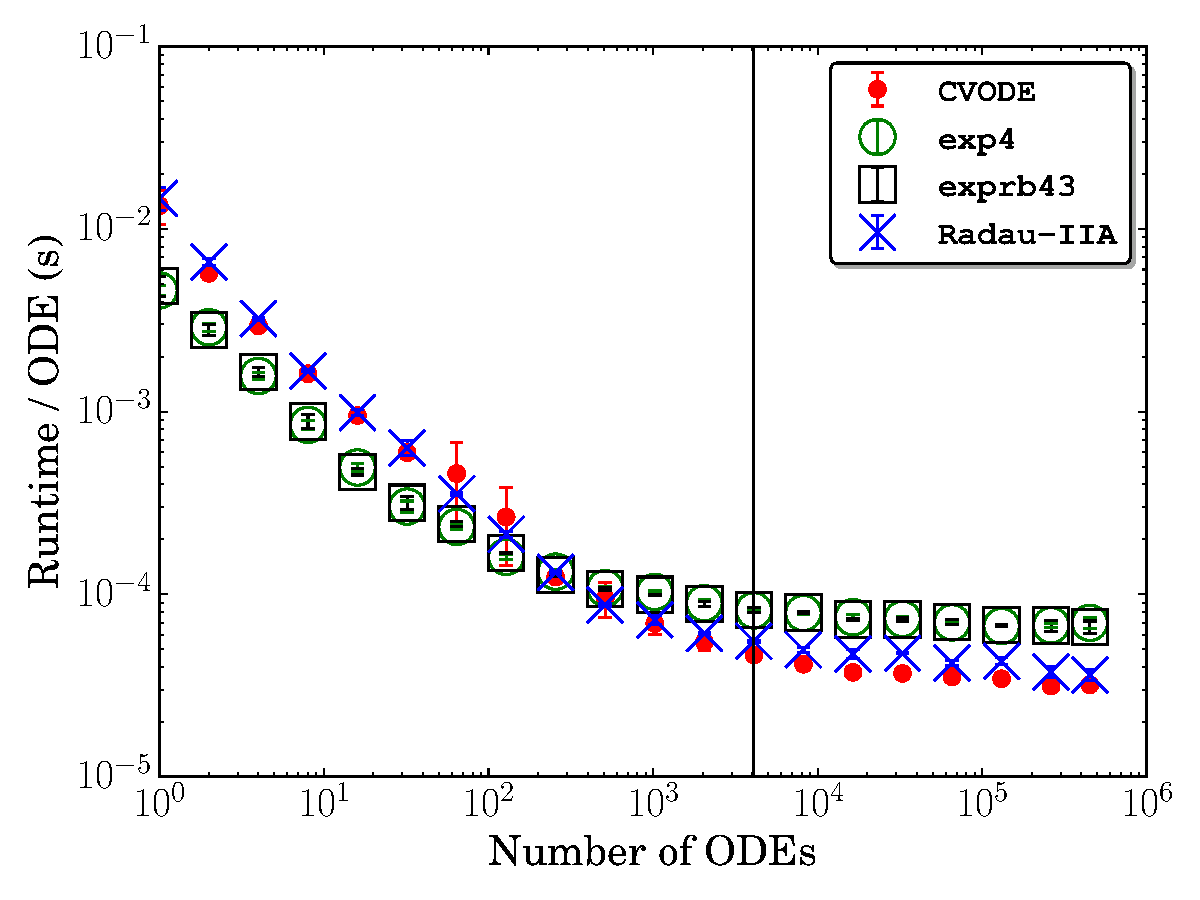
\includegraphics[width=\linewidth]{CH4_1e-06_cpu.pdf}
      \caption{CPU performance for $\delta t = \SI{e-6}{\second}$}
      \label{F:ch4_cpu_perf_small}
  \end{subfigure}
  %\hfill
  \begin{subfigure}{0.49\textwidth}
      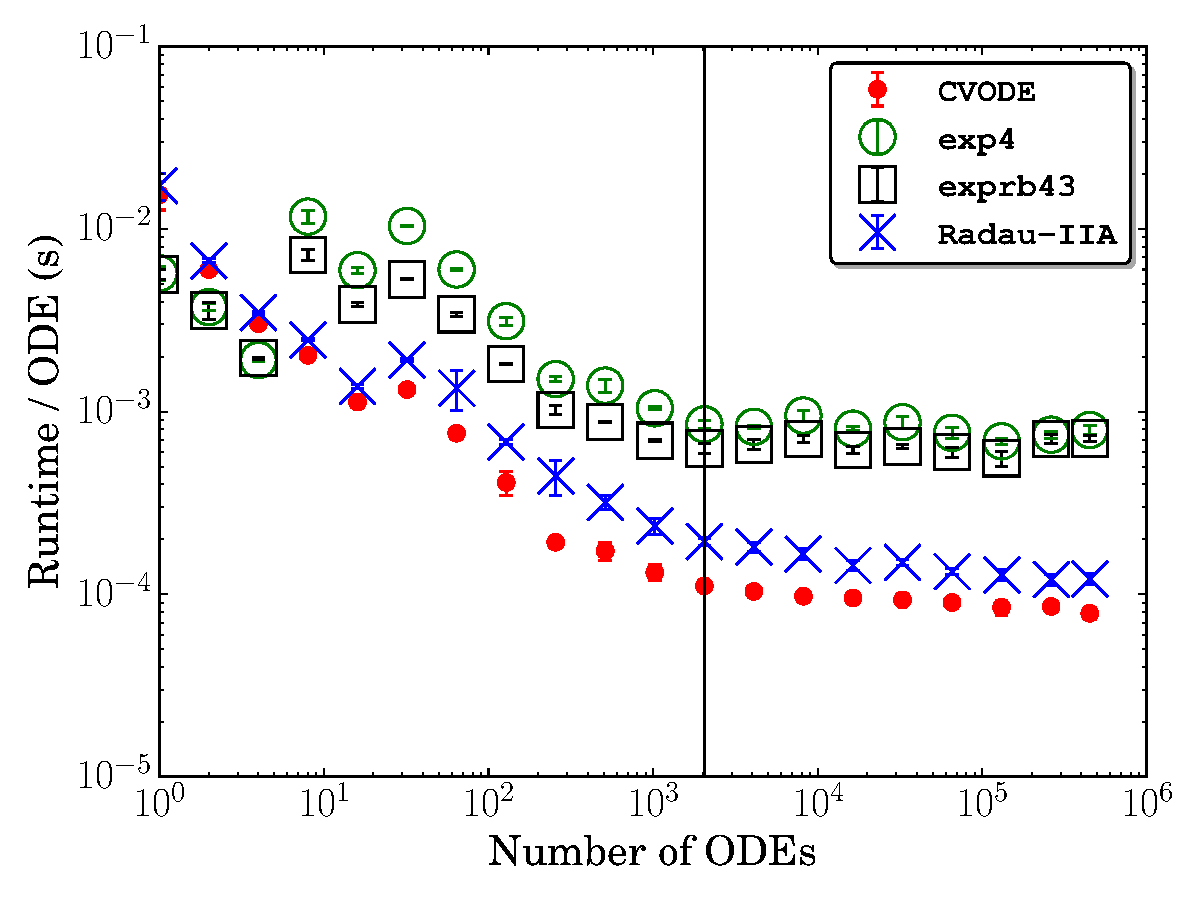
\includegraphics[width=\linewidth]{CH4_1e-04_cpu.pdf}
      \caption{CPU performance for $\delta t = \SI{e-4}{\second}$}
      \label{F:ch4_cpu_perf_large}
  \end{subfigure}\\
  \begin{subfigure}{0.49\textwidth}
      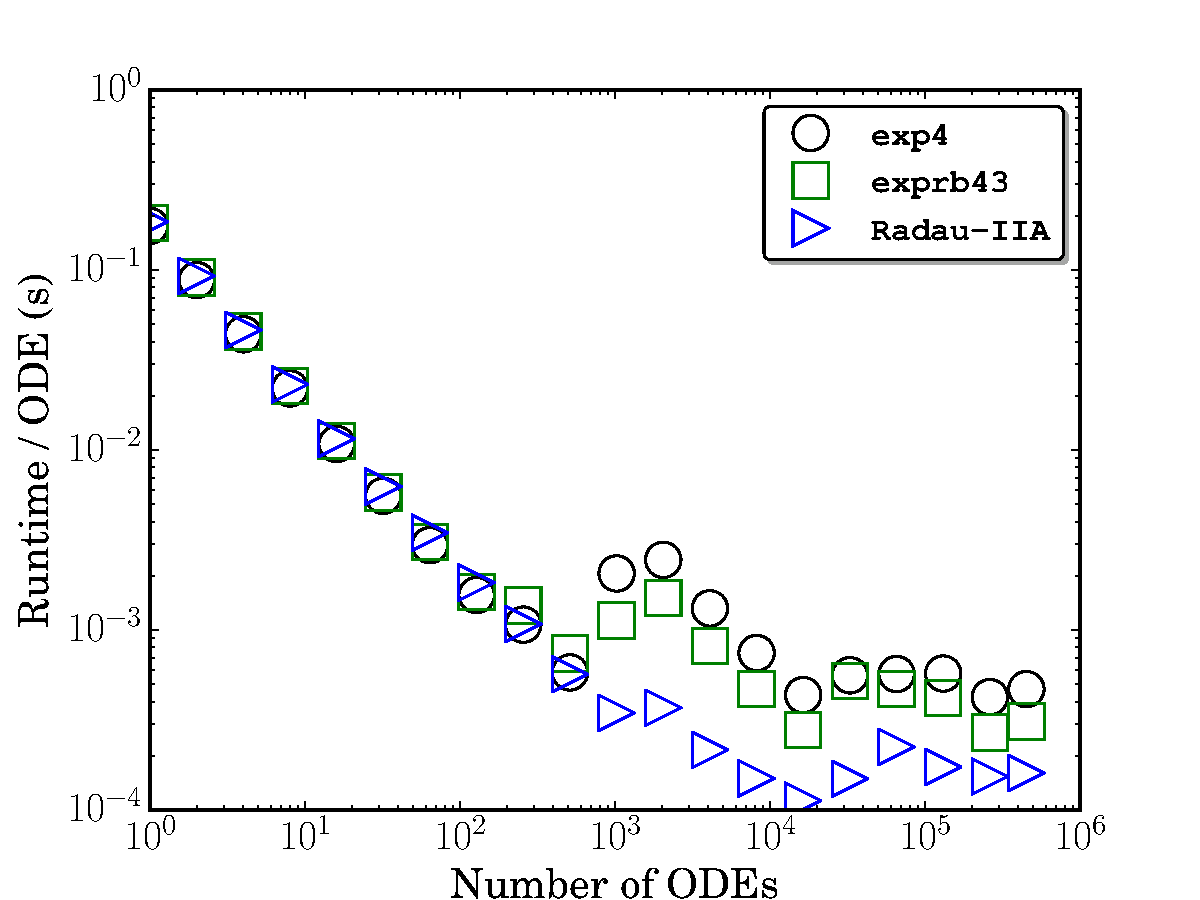
\includegraphics[width=\linewidth]{CH4_1e-06_gpu.pdf}
      \caption{GPU performance results for $\delta t = \SI{e-6}{\second}$}
      \label{F:ch4_gpu_perf_small}
  \end{subfigure}
  %\hfill
  \begin{subfigure}{0.49\textwidth}
      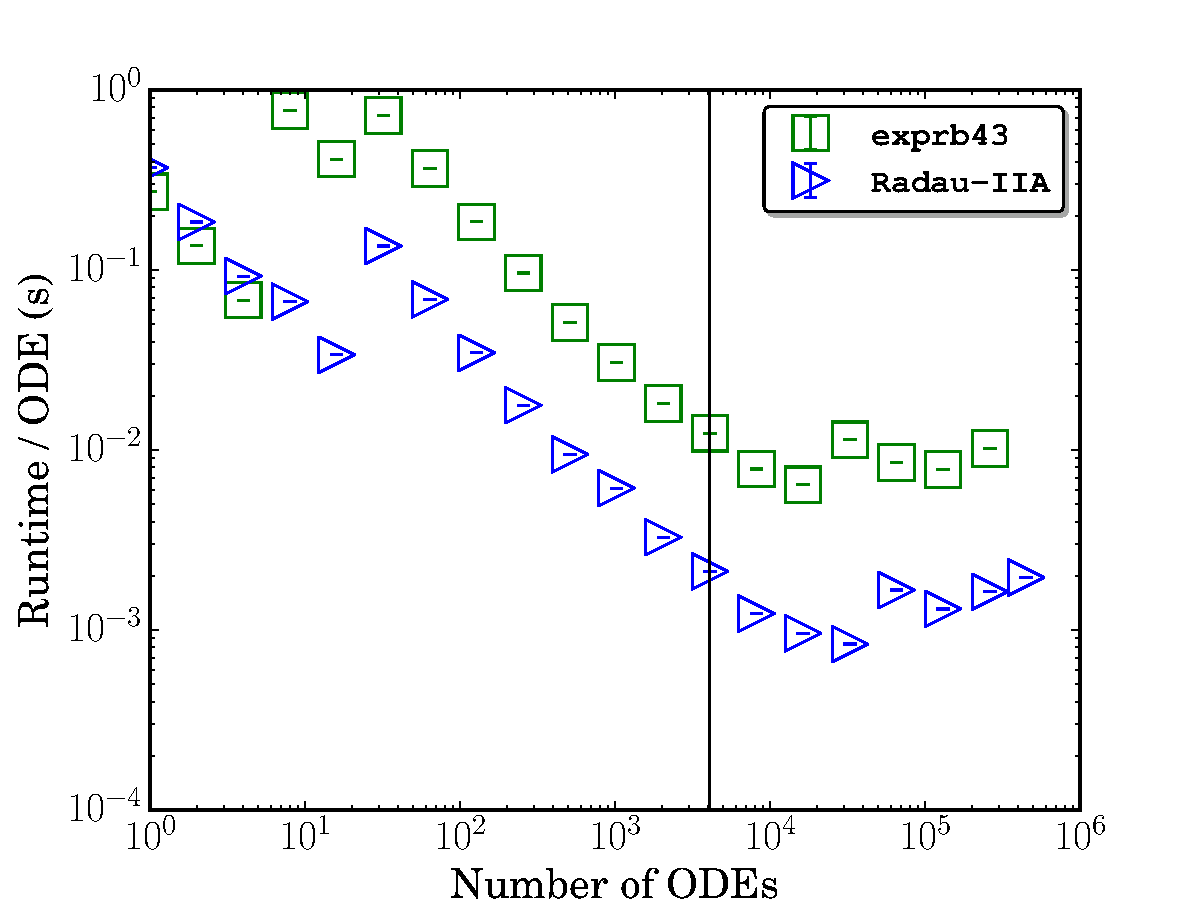
\includegraphics[width=\linewidth]{CH4_1e-04_gpu.pdf}
      \caption{GPU performance results for $\delta t = \SI{e-4}{\second}$}
      \label{F:ch4_gpu_perf_large}
  \end{subfigure}
  \caption{Average runtimes of the integrators, scaled by number of ODEs, on the CPU and GPU for the GRI-Mech 3.0 model at two different global time-step sizes.
  Estimation of where the runtime per ODE reaches a constant value (based on the results for \texttt{CVODE}\slash\texttt{Radau-IIA} for the CPU\slash GPU respectively) is marked in with a vertical line for all cases.
  Error bars indicate standard deviation.}
  \label{F:CH4_perf}
\end{figure}

Figure~\ref{F:CH4_perf} shows the runtime of the integrators for the GRI-Mech 3.0 model.
Similar to the \ce{H2}\slash\ce{CO} case for the smaller time-step, the CPU exponential integrators are more efficient (Fig.~\ref{F:ch4_cpu_perf_small}) for the near-equilibrium conditions at the beginning of the database.
For larger numbers of conditions, the implicit integrators are more efficient, and \texttt{CVODE} again performs the fastest.
Compared to the \ce{H2}\slash\ce{CO} model (Fig.~\ref{F:h2_cpu_perf_small}), the CPU-based implicit integrators perform significantly better than the exponential algorithms for the GRI-Mech 3.0 model with the small time-step (Fig.~\ref{F:ch4_cpu_perf_small}), which results from the higher stiffness present in the model.
This performance gap between the CPU implicit\slash exponential integrators increases for the larger time-step (Fig.~\ref{F:ch4_cpu_perf_large}) reaching nearly an order of magnitude difference in some cases.
Comparing the performance of the CPU implicit solvers between models shows roughly an order-of-magnitude performance decrease for both time-step sizes.
This phenomena, due largely to the increase in model size, is mostly mirrored by the \texttt{Radau-IIA} GPU solver for the smaller time-step size; the performance of which decreases by just over an order of magnitude.
However, for the larger time-step size, the GPU-based \texttt{Radau-IIA} solver performs roughly two orders of magnitude slower compared with the \ce{H2}\slash\ce{CO} case.
As will be examined in Sec.~\ref{S:divergence}, this dramatic decrease likely results from increased thread divergence in the \texttt{Radau-IIA} solver, as well as the increased memory traffic inherent in the larger model.

Unlike for the \ce{H2}\slash\ce{CO} model, the \texttt{exprb43} solver outperforms \texttt{exp4} for the GRI-Mech 3.0 model in all cases for the larger time-step size.
Although the \texttt{exprb43} and \texttt{exp4} algorithms each only require three exponential matrix function approximations per step, a single time step of \texttt{exprb43} is more expensive due to the extra chemical source term evaluations, matrix multiplications, and higher-order exponential matrix function requirement.
As such, the relatively simpler CPU \texttt{exp4} integrator outperforms the CPU \texttt{exprb43} integrator for the \ce{H2}\slash\ce{CO} model where there is relatively less chemical stiffness.
However, the nominal fourth-order convergence of the \texttt{exp4} algorithm is a classical nonstiff order, and thus order reduction is expected for stiff problems~\cite{ANU:7701740,Bisetti:2012jw}.
Correspondingly, for the larger time-step GRI-Mech 3.0 case, \texttt{exprb43} typically outperforms \texttt{exp4} on both the CPU and GPU.


% The GPU \texttt{Radau-IIA} integrator outperformed \texttt{CVODE} for the smaller time-step size; at best, it ran \SI{31.5}{\percent} faster than \texttt{CVODE} (\num{131072} ODEs), and at worst was \SI{10}{\percent} faster (\num{16384} ODEs).
% The larger time-step size again negatively impacted the performance of the GPU-based \texttt{Radau-IIA} integrator, dropping the performance to \num{8.63}$\times$ slower than \texttt{CVODE} at best (\num{32768} ODEs), and \num{20.5}$\times$ slower in the worst case (\num{450900} ODEs).
% For the smaller time-step size the CPU \texttt{Radau-IIA} integrator was \SI{13}{\percent} faster than \texttt{CVODE} at best (\num{131072} ODEs) and \SI{10}{\percent} faster at worst (\num{450900} ODEs).
% The larger time-step size---the stiffest case---was the only case where \texttt{CVODE} significantly outperformed CPU \texttt{Radau-IIA}, which was \num{2.66}$\times$ slower at best (\num{65536} ODEs) and \num{4.11}$\times$ slower at worst (\num{450900} ODEs).
% This difference may be due to the adaptive-order nature of the \texttt{CVODE} algorithm, or potentially due to its maturity and years of optimization.
% However, this effect is fairly minor and should not cause the order-of-magnitude decrease in relative performance between the GPU-based \texttt{Radau-IIA} integrator and \texttt{CVODE} observed when switching to the larger time step.

\subsection{CPU\slash GPU performance comparison}

Meaningful performance comparison between CPU\slash GPU based integration presents challenges for several reasons.
First, the vastly different nature of the processing cores between platforms eliminates the possibility of normalized performance comparison by core count.
Further, unlike many common GPU-accelerated applications where the number of operations required to solve the problem is known (e.g., as in linear-algebra operations, or fast Fourier transforms), the floating operation (FLOP) count required for chemical kinetic integration is not so readily available, precluding performance comparison on a FLOP per second basis.
Although the runtimes of the GPU integration algorithms can be directly compared with that of the CPU based solvers, these figures are not particularly informative.
For instance, if a GPU algorithm is $\SI{10}{\times}$ faster than the equivalent algorithm on two six-core CPUs, how does this compare to two eight-core CPUs, etc.?

For researchers in numerical combustion, two issues stand out as particularly important for performance evaluation: runtime and cost.
As established in Section~\ref{sec:Intro}, large-scale reacting flow simulations with realistic chemical kinetic models are extremely computationally expensive, and remain outside of the capabilities of most in the field.
With this in mind, we ask, for a given large-scale reacting flow simulation, what is the effect on the overall runtime of adding more CPU cores compared with adding GPU accelerators?
In addition, if a budget is allocated to expand available computational resources, how might these funds be best allocated?
To answer these questions, we attempt to derive a rough estimate of the number of CPU cores required for equivalent performance on the GPU.

A nominal performance metric for both the CPU- and GPU-based integration algorithms must first be obtained.
As the most efficient solvers in all cases are \texttt{CVODE} for the CPU, and \texttt{Radau-IIA} for the GPU, these algorithms will be considered as the performance benchmarks.
Furthermore, most large-scale simulations consist of millions of cells (or more), and therefore we only consider the performance limit of each algorithm (i.e., the cost per ODE of each algorithm in the region where this cost reaches an approximately constant value).
To this end, Figs.~\ref{F:H2_perf} and \ref{F:CH4_perf} show vertical lines in all cases where the runtime per ODE first reaches within \SI{10}{\percent} of its final value\todo{may want to explain this}~(based on \texttt{CVODE}\slash\texttt{Radau-IIA} for the CPU\slash GPU accordingly).
The cost per ODE above and including these thresholds has been averaged and forms our nominal performance measure.
The CPU performance measure must also be normalized by the total number of cores used: \num{40}.
The ratio of these performance measures can give a rough estimate of the number of CPU cores required to equal the GPU performance for the cases studied, and are presented in Table~\ref{T:cpu_equiv}.
For all but the GRI-Mech 3.0 case with the larger time-step size, the GPU is roughly equivalent to \num{10} or more CPU cores and up to $\sim$\num{35} cores for the \ce{H2}\slash\ce{CO} case with the smaller time-step size.
Finally, at the time of writing, the ten-core Intel Xeon E5-4640 v2 CPU used in this study is listed for a recommended customer price of \SI{2725}[\$]{}, while a new Tesla C2075 GPU is available for $\sim$\SI{1400}[\$]{}\todo{{[}citations needed{]}, including dates}.
These prices are only rough estimates of the actual cost of these devices, e.g., the actual price for the Intel CPU may be significantly less in a configured server node, while the Tesla C2075 is no longer sold directly by NVIDIA, and thus the prices are variable.
Furthermore, the performance decrease using an older, cheaper CPU (e.g., the Intel Xeon X5650 used as host processor for the GPU simulations in this work) may not be that large.
However, combined with the equivalent core counts in Table~\ref{T:cpu_equiv}, this information suggests that the Tesla C2075 is a reasonable investment to supplement computing power for chemical-kinetic integration in large-scale large-eddy simulations.
For the time-step size of \SI{e-4}{\second}, corresponding to Reynolds-averaged simulations, the benefit is less clear for the stiffer GRI-Mech 3.0 model; more work is required in thread divergence avoidance and memory traffic reduction to improve the performance in this case.


\begin{table}[htb]
\centering
\begin{tabular}{@{}l S[table-format=2.1] S[table-format=2.1] @{}}
\toprule
\multirow{2}{*}{Time-step size} & \multicolumn{2}{c}{\# equivalent CPU cores} \\ \cmidrule{2-3}
 & \ce{H2}\slash\ce{CO} & \ce{CH4} \\
\midrule
\SI{e-6}{\second} & 35.3 & 10.5 \\
\SI{e-4}{\second} & 14.1 & 2.6 \\
\bottomrule
\end{tabular}
\caption{The number of CPU cores (roughly) required for equivalent performance to a single GPU for the combinations of chemical kinetic models and time-step sizes studied.}
\label{T:cpu_equiv}
\end{table}


\subsection{Effect of thread divergence}
\label{S:divergence}

Thread divergence and memory traffic are two performance concerns particularly important for chemical kinetic integration on SIMD platforms.
Slowdown due to memory traffic for a GPU integration algorithm implemented on a per-thread basis primarily results from the small amount of on-chip memory available.
Reformulating the chemical kinetic equations to generate sparse Jacobian matrices~\cite{Schwer2002270} would likely benefit GPU-based integration algorithms due to the reduced memory requirements; this is a planned improvement to the \texttt{pyJac} software~\cite{Niemeyer:2016aa,niemeyer_2016_51139}.
The performance penalty due to thread divergence depends both on the cost of the divergent branches as well as the proportion of the warp that executes each branch.
For example, if only one thread in a warp executes an expensive branch (e.g., a Jacobian update) the rest of the warp remains idle during that time, and the SM may become underutilized.

To investigate the effects of thread divergence further, we adopted a similar quantification of thread divergence to that of Niemeyer and Sung~\cite{Niemeyer:2014aa}:
\begin{equation}
	D = \frac{\sum_{i=1}^{32}{d_i}}{32 \times \max\limits_{i = 1, \dots, 32} d_i} \;,
	\label{eqn:divergence}
\end{equation}
where $d_i$ is the number of internal integrator time steps taken to reach the global time step by thread $i$ in a warp (which consists of 32 threads).
$D$ represents the similarity of internal time step counts across threads in a warp---a significant source of thread divergence.
If all threads in a warp use identical internal integration time steps and thus the warp experiences no thread divergence from this source, then $D = 1$; however, if a warp experiences an unbalanced number of internal integration time steps, then $D \to 0$.
Differing time-step sizes is not the only source of thread divergence for the GPU integration algorithms.
For instance, threads in a warp may use different Krylov subspace sizes for the exponential integrators or different numbers of Newton iterations for the \texttt{Radau-IIA} solver.
Indeed, Sec.~\ref{S:results} notes that we suspect thread divergence from differing Krylov subspace sizes as the reason the exponential solvers are less efficient for small numbers of ODEs for the \ce{H2}\slash\ce{CO} model with the small time-step size.
However, the cost of these operations are clearly less than that of an entire internal integration step (in which they are embedded) and thus we look only at the thread divergence of internal integration time steps.
Investigation of thread divergence for such operations within a internal integration step is an important consideration and will be explored in our future work.

\begin{figure}[htb]
  \centering
  \begin{subfigure}{0.49\textwidth}
      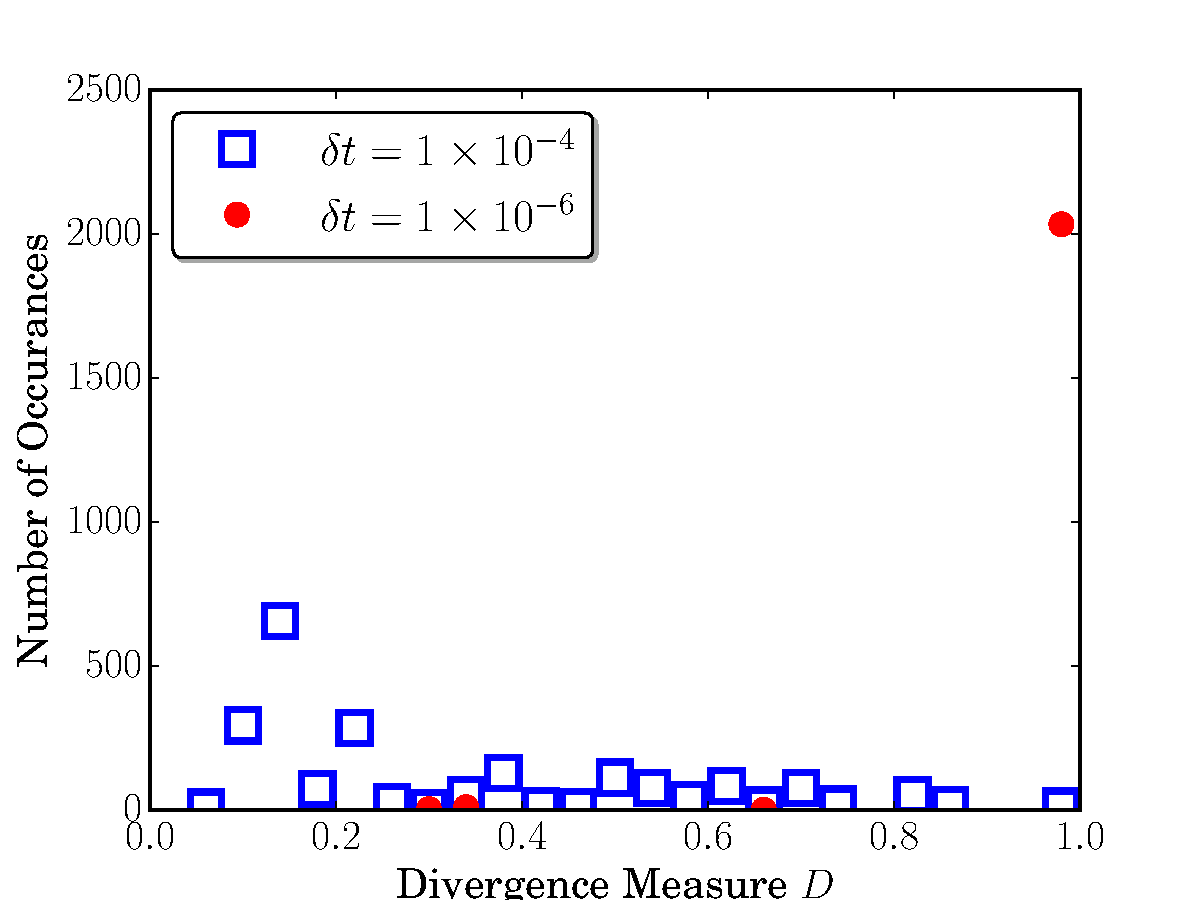
\includegraphics[width=\linewidth]{H2_radau2a_div.pdf}
      \caption{\ce{H2}\slash\ce{CO} model}
  \end{subfigure}
  %\hfill
  \begin{subfigure}{0.49\textwidth}
      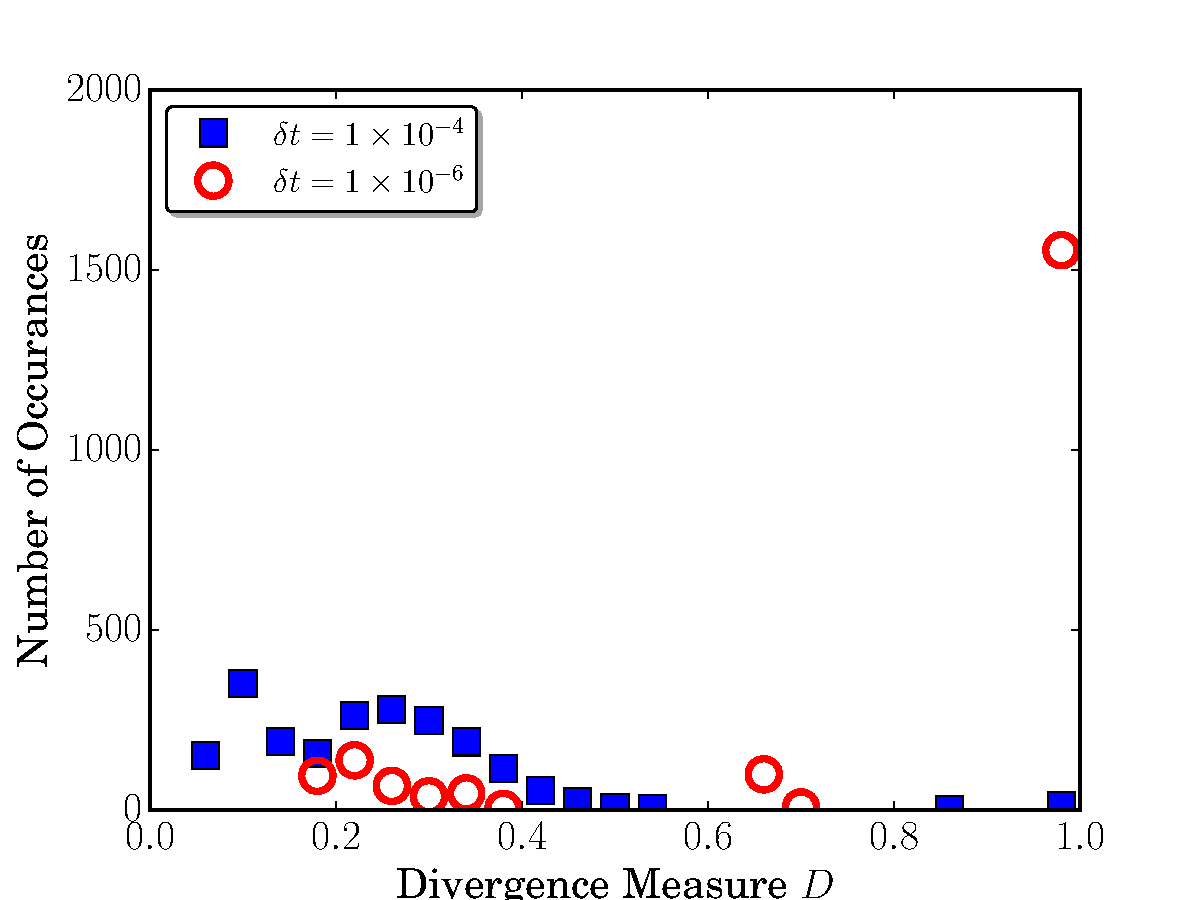
\includegraphics[width=\linewidth]{CH4_radau2a_div.pdf}
      \caption{GRI-Mech 3.0 model}
      \label{F:Rad_div_gri}
  \end{subfigure}
  \caption{Thread divergence estimate for the \texttt{Radau-IIA} solver for both models and time-step sizes.}
  \label{F:rad_divergence}
\end{figure}
\begin{figure}[htb]
  \centering
  \begin{subfigure}{0.49\textwidth}
      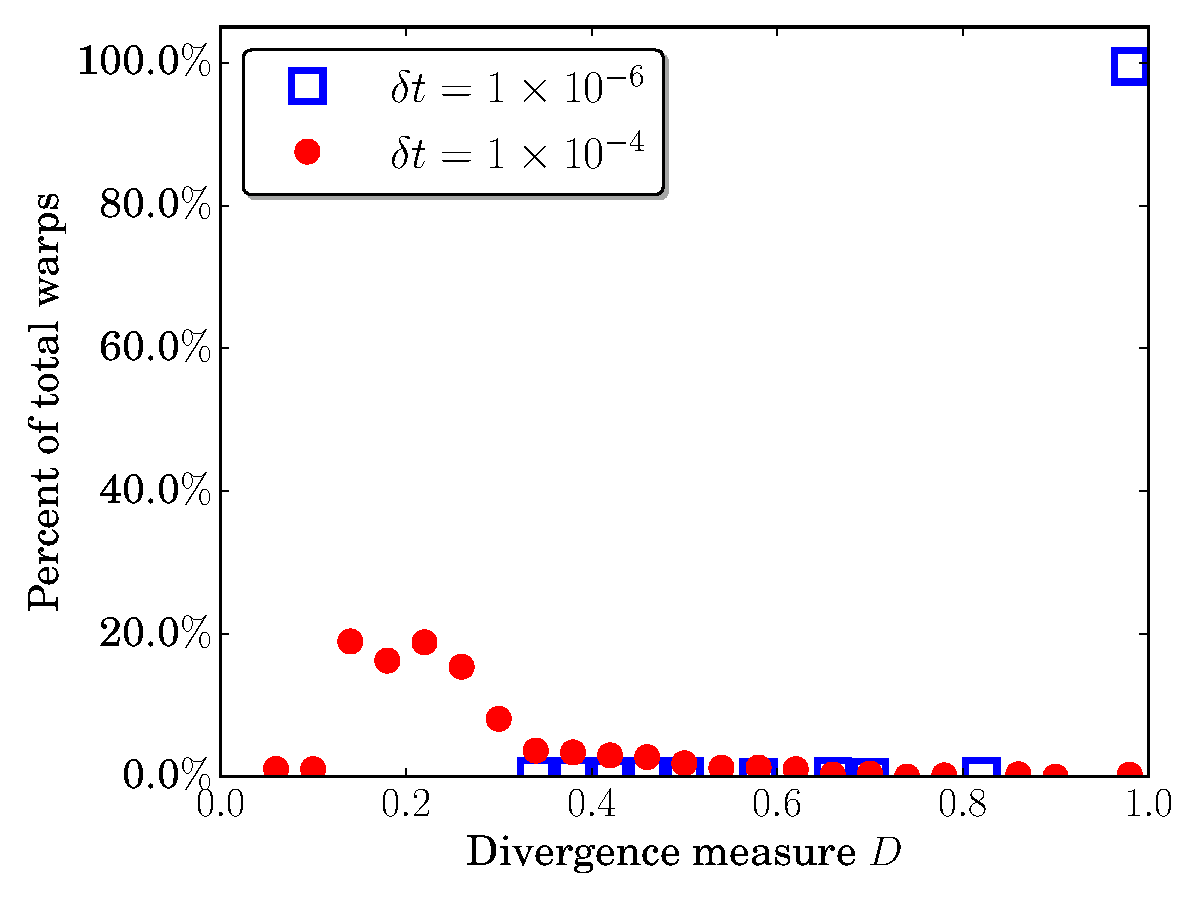
\includegraphics[width=\linewidth]{H2_exprb43_div.pdf}
      \caption{\ce{H2}\slash\ce{CO} model}
  \end{subfigure}
  %\hfill
  \begin{subfigure}{0.49\textwidth}
      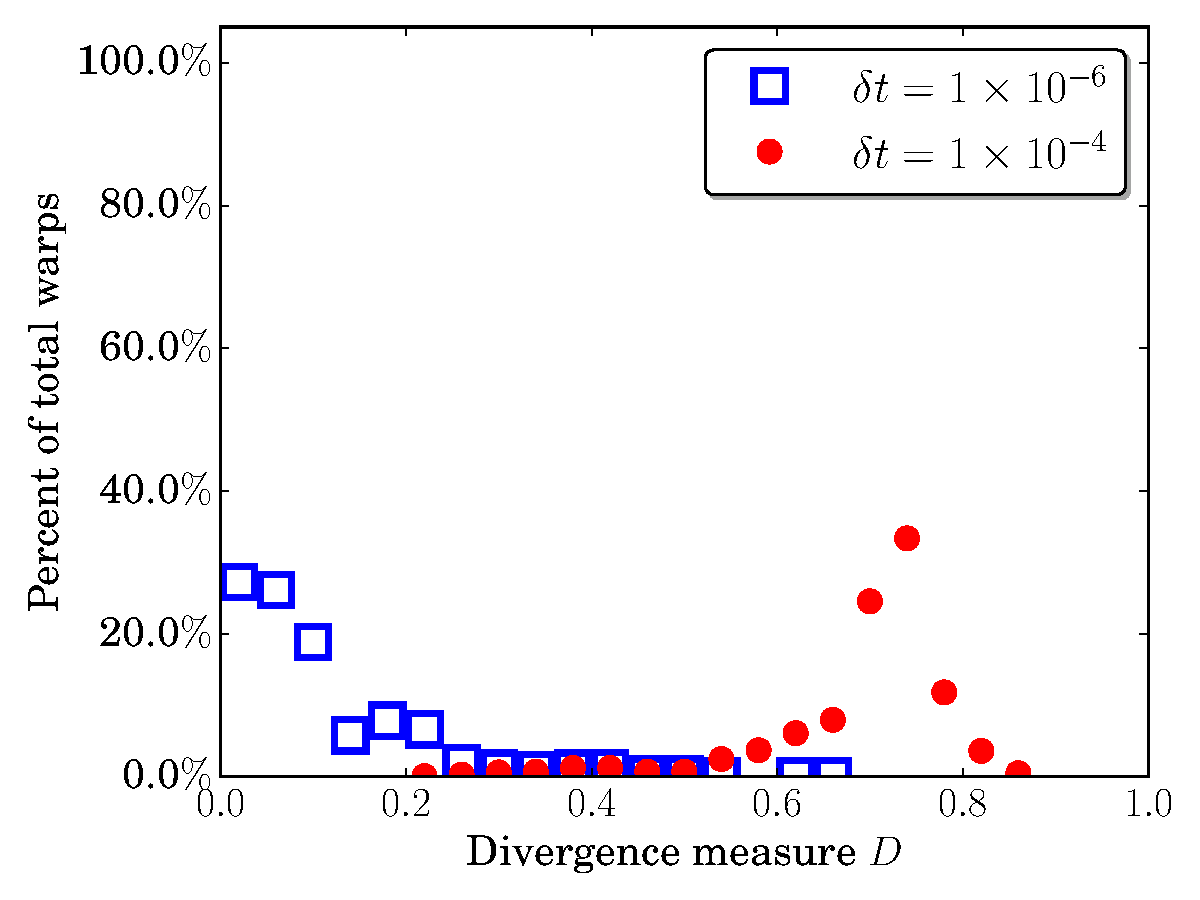
\includegraphics[width=\linewidth]{CH4_exprb43_div.pdf}
      \caption{GRI-Mech 3.0 model}
  \end{subfigure}
  \caption{Thread divergence estimate for the \texttt{exprb43} solver for both models and time-step sizes.}
  \label{F:exp_divergence}
  \todo[inline]{Why only two models? Where's exp4?}
\end{figure}

Figure~\ref{F:rad_divergence} shows the distribution of the divergence measure $D$ for the \texttt{Radau-IIA} solver with both time-step sizes and kinetic models when run on \num{262144} ODEs, spread across \num{8192} warps.
For both kinetic models, increasing the global  integration time-step size resulted in a sharp increase in the number of warps with high levels of thread divergence (i.e., $D < 0.5$).
The approximate equivalent CPU core-count (Table~\ref{T:cpu_equiv}) correspondingly drops to \SIrange{2.5}{4}{$\times$}.
Furthermore, the GRI-Mech 3.0 model experiences higher levels of thread divergence for the larger time-step size, and subsequently exhibits a larger drop in performance compared with the \ce{H2}\slash\ce{CO} model.
Thread divergence may be an even more important concern for chemical kinetic models with high chemical stiffness\todo{aren't we supposed to be considering stiff chemistry in this paper?}.
This observation motivates future work aimed at developing strategies to reduce thread divergence.
Potential solutions include adopting an ODE per-block approach~\cite{Stone:2013aa}, reordering ODEs to increase similarity of stiffness inside a warp, or synchronizing time-step sizes between threads in a warp.
However, Fig.~\ref{F:rad_divergence} does not explain the drop in equivalent core count between the \ce{H2}\slash\ce{CO} model and the GRI-Mech 3.0 model for the smaller time-step size.
This likely results from a combination of thread divergence inside the internal integration step and the increased memory traffic of the larger model; this further motivates development of a sparse version of the \texttt{pyJac} software.

Figure~\ref{F:exp_divergence} shows the divergence levels of the \texttt{exprb43} GPU solver.
Similar to the \texttt{Radau-IIA} solver, both models show only minor levels of thread divergence due to differing internal integration step sizes for the smaller time-step size.
For the larger time-step size, greatly increased levels of thread divergence are observed for both models.
This differs from the behavior of the \texttt{Radau-IIA} solver, which only shows high thread divergence for the GRI-Mech 3.0 model.
This is expected as the explicit solvers are less efficient at dealing with stiffness, and end up using a greater range of time-step sizes between stiff and non-stiff conditions.

\subsection{Effect of using a finite-difference-based chemical kinetic Jacobian}

While it is well established that using an analytical Jacobian matrix can significantly accelerate chemical kinetic integration on the CPU~(e.g., \cite{Lu:2009gh,stone2014comparison,Schwer2002270}), to our knowledge no work using an analytical Jacobian for GPU-based chemical kinetic integration has been published.\todo{what about Dijkmans et al. paper?}
To this end, in this section we explore using a first-order finite-difference-based Jacobian matrix on the GPU and compare the relative performance benefits of the analytical Jacobian with those achieved on the CPU.\todo{this sentence is confusing, needs some work}
The exponential methods require an exact Jacobian matrix (rather than an approximation as given by finite-difference methods), so we did not consider their performance in this section.

Figure~\ref{F:AJ_comp} shows the speedup achieved on both the CPU and GPU for the \texttt{Radau-IIA} algorithm for various cases.
For the \ce{H2}\slash\ce{CO} model (Figs.~\ref{F:AJ_h2_small} and~\ref{F:AJ_h2_large}), using the analytical Jacobian offers minimal performance benefit for the CPU-based integrators, reaching speedups of only $\mathcal{O}(\num{1}\times)$ for both time-step sizes.
This results from both the relatively small size of the model (and resulting modest chemical source-term evaluation costs), as well as the lower chemical stiffness that requires only a few Jacobian evaluations for the \texttt{Radau-IIA} solver.
In some cases the finite-difference Jacobian solver is faster than the analytical Jacobian solver; although difficult to explain the exact cause of this phenomena, it is likely that differences in the finite-difference Jacobian caused the integrator to follow a slightly different path (e.g., with fewer Jacobian updates\slash chemical source term evaluations) changing the integration cost.
However, for large numbers of conditions, the analytical-Jacobian-based solver indeed performs faster than the finite-difference counterpart.\todo{some numbers here please}
In contrast, the analytical-Jacobian-based GPU solver performs significantly faster\todo{numbers here too} than the finite-difference GPU solver in all cases for the \ce{H2}\slash\ce{CO} model.
As discussed in Sec.~\ref{S:divergence}, significantly higher levels of thread divergence are expected for the larger time-step size.
The GPU-based solver achieves corresponding maximum speedups of $\mathcal{O}(\num{10}\times)$ and $\mathcal{O}(\num{100}\times)$ for the smaller and larger time-step sizes, respectively.
Figure~\ref{F:AJ_ch4_small} shows that the speedup for the CPU solver reaches \SIrange{2}{3}{$\times$} for the larger, more stiff GRI-Mech 3.0 model at the smaller time-step size.
Similar to the \ce{H2}\slash\ce{CO} case with the smaller time-step, the analytical-Jacobian-based GPU \texttt{Radau-IIA} solver performs $\mathcal{O}(10\times)$ faster for the GRI-Mech 3.0 Model.\todo{maybe give specific numbers rather than orders in this section?}

\begin{figure}[htb]
  \centering
  \begin{subfigure}{0.49\textwidth}
      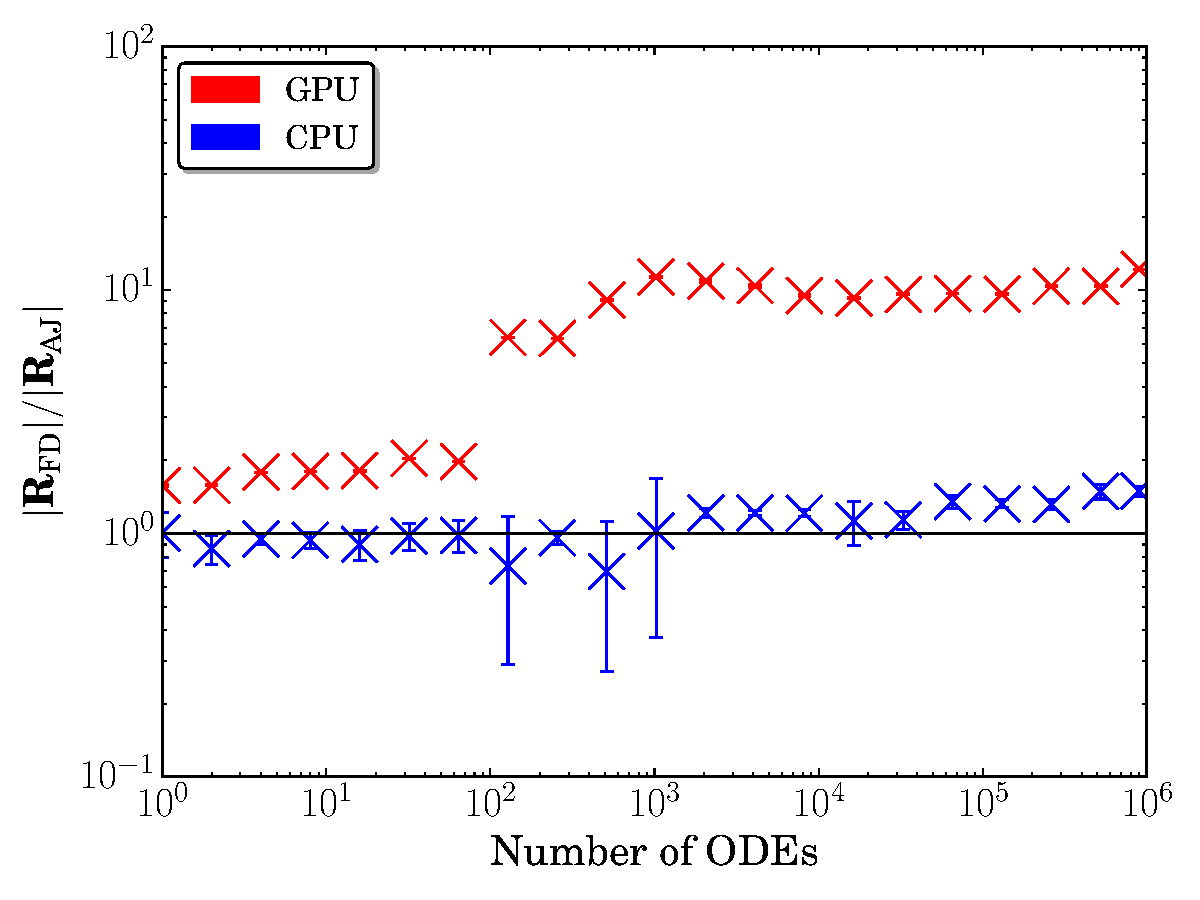
\includegraphics[width=\linewidth]{H2_1e-06_ajac_comp.pdf}
      \caption{\ce{H2}\slash\ce{CO} model with $\delta t = \SI{1e-6}{\second}$}   
      \label{F:AJ_h2_small}
  \end{subfigure}
  %\hfill
  \begin{subfigure}{0.49\textwidth}
      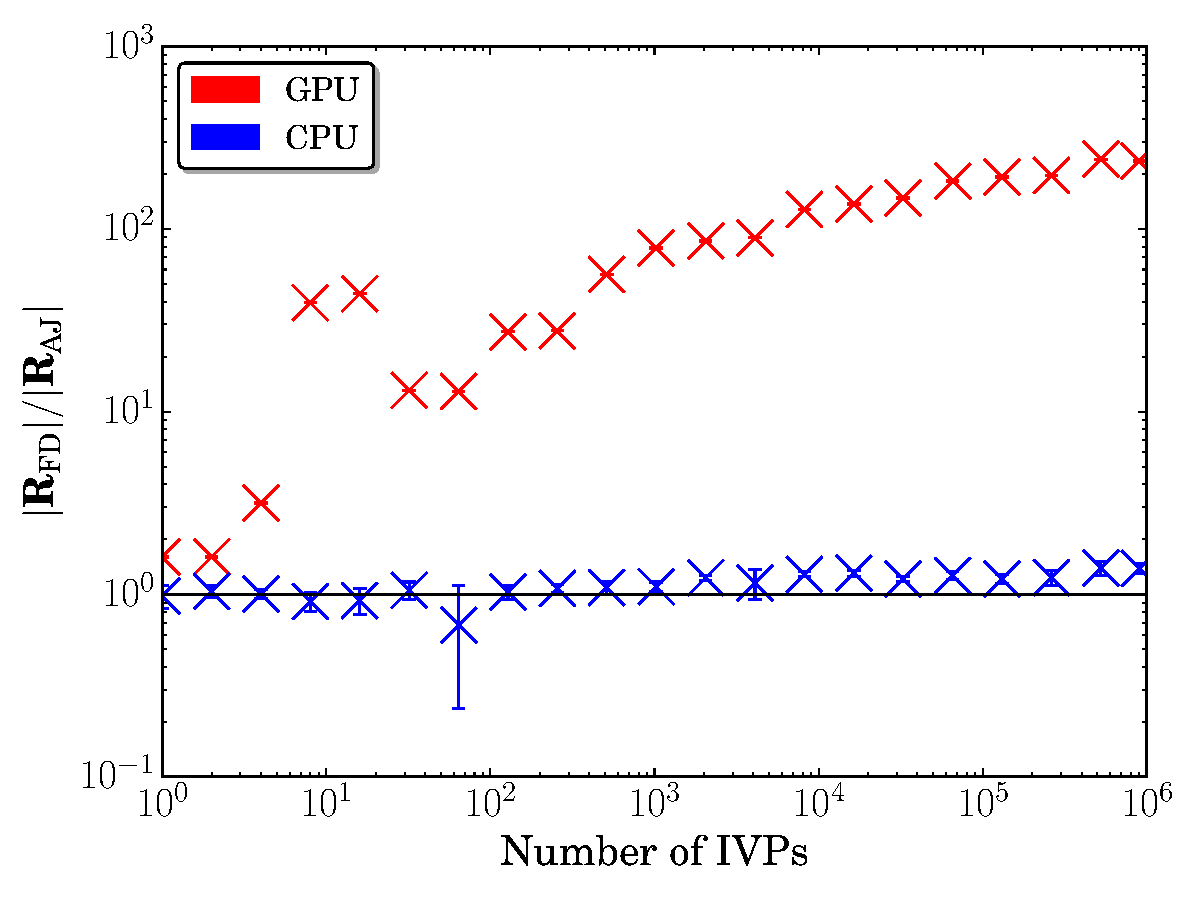
\includegraphics[width=\linewidth]{H2_1e-04_ajac_comp.pdf}
      \caption{\ce{H2}\slash\ce{CO} model with $\delta t = \SI{1e-4}{\second}$}
      \label{F:AJ_h2_large}
  \end{subfigure}
  \\
  \begin{subfigure}{0.49\textwidth}
      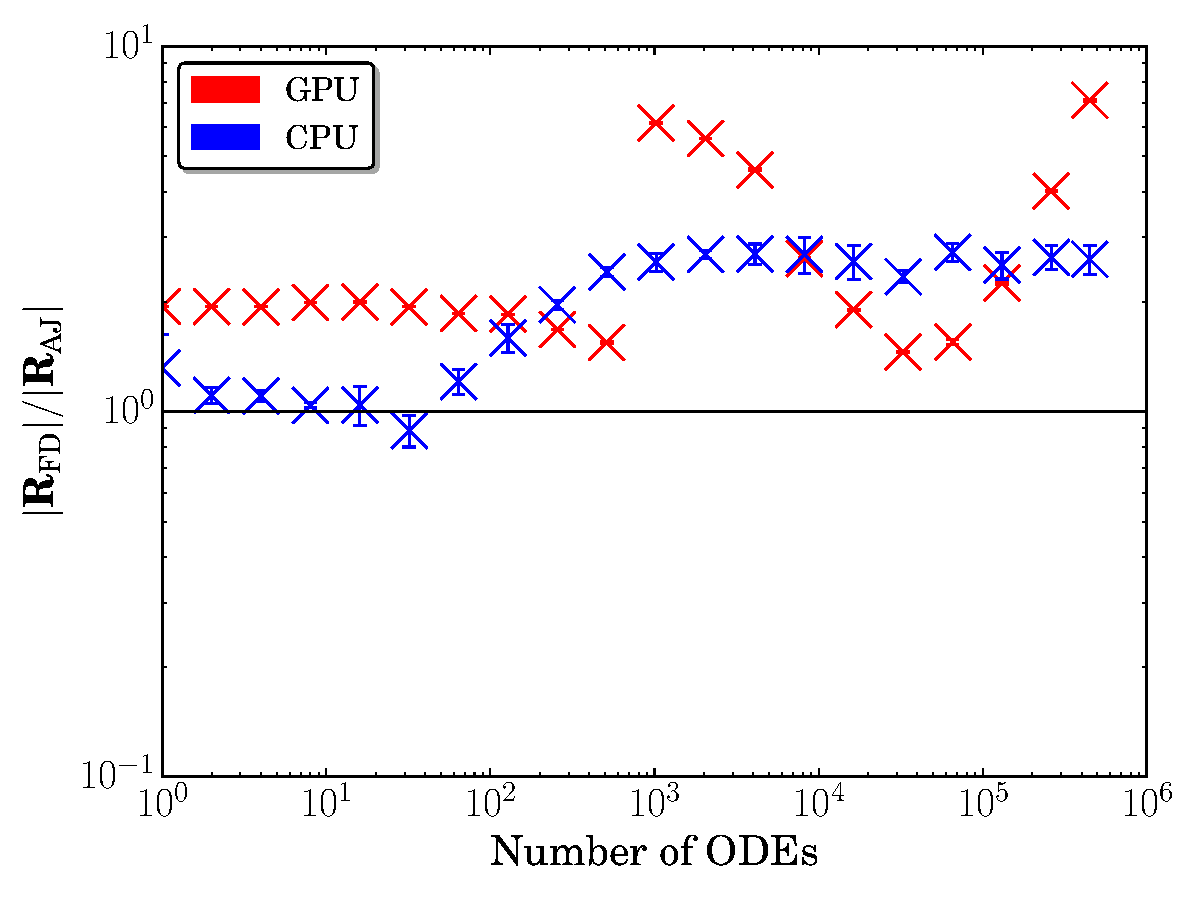
\includegraphics[width=\linewidth]{CH4_1e-06_ajac_comp.pdf}
      \caption{GRI-Mech 3.0 model with $\delta t = \SI{1e-6}{\second}$}
      \label{F:AJ_ch4_small}
  \end{subfigure}
  \caption{Ratio of the average finite-difference Jacobian based integrator runtime $\lvert\textbf{R}_{\text{FD}}\rvert$ to that of the analytical Jacobian runtime $\lvert\textbf{R}_{\text{AJ}}\rvert$ for the \texttt{Radau-IIA} (CPU\slash GPU) solvers.
  Error bars indicate standard deviation, and the horizontal lines show a ratio of one.}
  \label{F:AJ_comp}
\end{figure}

% \subsection{Effect of shared memory caching}
% \label{S:smem}
% 
% The effectiveness of the shared memory caching scheme was evaluated in several cases by comparing the mean runtime of the integrators using chemical source terms and analytical Jacobian subroutines generated with and without the caching algorithm enabled.
% We observed typical speedups of $\SI{5}{\percent}$ and $\SI{10}{\percent}$ for the smaller and larger global time-step sizes, respectively.
% This difference resulted from an increase in chemical source term and Jacobian evaluations required for the larger time-step size cases.
% Even larger speedup factors were observed in certain cases with the GRI-Mech 3.0 model: a \SI{24.4}{\percent} speedup with \texttt{exp4} for \num{131072} ODEs and the \SI{e-6}{\second} time-step size, and a \SI{13.2}{\percent} speedup with \text{Radau-IIA} for \SI{32768} ODEs and the \SI{e-4}{\second} time-step size.
% Thus, we recommend using this or a similar caching scheme in order to exploit shared memory in GPU integrators implemented on a per-thread basis.


%%%%%%%%%%%%%%%%%%%%%%%%%%%%%%%%%%%%%%%%%%%%
\section{Conclusions}
\label{S:conclusions}
%%%%%%%%%%%%%%%%%%%%%%%%%%%%%%%%%%%%%%%%%%%%

The large size and chemical stiffness of chemical kinetic models for fuels relevant to transportation and power generation applications traditionally requires the use of high-order implicit integrators for efficient solutions.
Past work showed orders-of-magnitude speedups for solution of nonstiff to moderately stiff chemical kinetic systems using explicit solvers on GPUs.\todo{add refs}
In contrast, work on stiff chemical kinetic integration with implicit GPU solvers has been limited to specialized cases, or failed to surpass current CPU-based techniques.

This work demonstrated the performance of GPU-based integration methods capable of handling greater stiffness, including an implicit fifth-order Runge--Kutta algorithm and two fourth-order exponential integration algorithms, using chemical source term and analytical Jacobian subroutines provided by the \texttt{pyJac} software~\cite{niemeyer_2016_51139,Niemeyer:2015ws,Niemeyer:2016aa}.
For time-step sizes relevant to large-eddy simulations of turbulent combustion, the GPU-based implicit Runge--Kutta method compared favorably with the CPU-based implicit \texttt{CVODE} integrator for both chemical kinetic models studied.
For longer time-step sizes, the performance of all GPU solvers decreased significantly due to increased levels of thread divergence.
The exponential solvers performed significantly worse than \todo{than what? Radau, cvode, both?} in all relevant cases.
Based on these results, we conclude that the higher levels of thread divergence present for the exponential solvers combined with the relatively high cost of integration steps due to Arnoldi iteration (as compared to other explicit integration techniques) make them a poor fit for SIMD acceleration.
Instead, further focus on stiff explicit solvers should be directed towards (non-exponential) Rosenbrock solvers and inexact Jacobian W-methods, as explored for the CPU by Stone and Bisetti~\cite{stone2014comparison}.
We found that using an analytical Jacobian matrix on the GPU is critical to efficient chemical kinetic integration, with the performance benefits thereof greatly surpassing those achieved by using an analytical Jacobian on the CPU.
Finally, thread divergence and memory traffic were identified as key performance concerns for GPU chemical kinetic integration algorithms.
\todo[inline]{maybe lay out our main conclusions and contributions as a bulleted list, instead of paragraph form? That helps people grab the main takeaways.}
\todo[inline]{also, may be good to add some specific numbers here}

Further improvements to the analytical Jacobian code, e.g., by using a chemical kinetic system based on species concentrations to increase Jacobian sparsity, are likely to further increase performance of the developed algorithms.
However, this work clearly showed that thread divergence poses a large challenge to high performance of GPU-based integration techniques on a per-thread basis.
Our future work will therefore focus on a more comprehensive study of thread divergence, as well as developing methods to mitigate or eliminate its negative performance impact.
Finally, new integration techniques such as hybrid implicit\slash explicit solvers and explicit non-exponential Rosenbrock algorithms will be investigated and paired with work studying the selection of appropriate solvers based on estimated chemical stiffness.


%%%%%%%%%%%%%%%%%%%%%%%%%%%%%%%%%%%%%%%%%%%%%%%%%%%%%%%%%%%%%%%%%%%%%%
\section*{Acknowledgments}

This material is based upon work supported by the National Science Foundation under grants ACI-1534688 and ACI-1535065.

%% The Appendices part starts with the command \appendix;
%% appendix sections are then done as normal sections
\appendix
\setcounter{figure}{0}

% Fix for missing space between "Appendix" and letter
\renewcommand*{\thesection}{\appendixname~\Alph{section}}

%%%%%%%%%%%%%%%%%%%%%%%%%%%%%%%%%%%%%
\section{Raw Performance Data Plots}
%%%%%%%%%%%%%%%%%%%%%%%%%%%%%%%%%%%%%
\label{S:raw}

In this section we present the plots of the raw performance data for completeness, as described in Sec.~\ref{S:results}.

\begin{figure}[htb]
  \centering
  \begin{subfigure}{0.49\textwidth}
      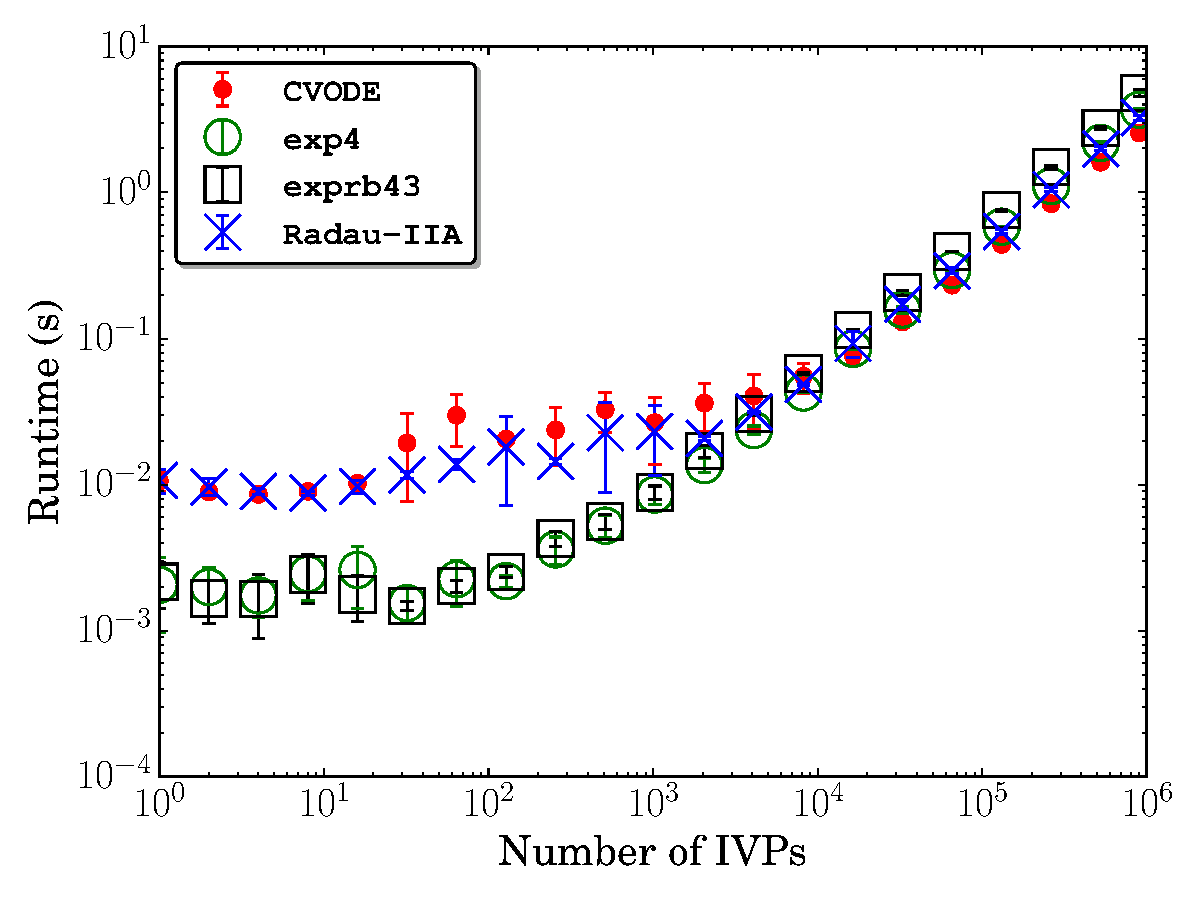
\includegraphics[width=\linewidth]{H2_1e-06_cpu_nonorm.pdf}
      \caption{CPU performance for $\delta t = \SI{e-6}{\sec}$}
  \end{subfigure}
  %\hfill
  \begin{subfigure}{0.49\textwidth}
      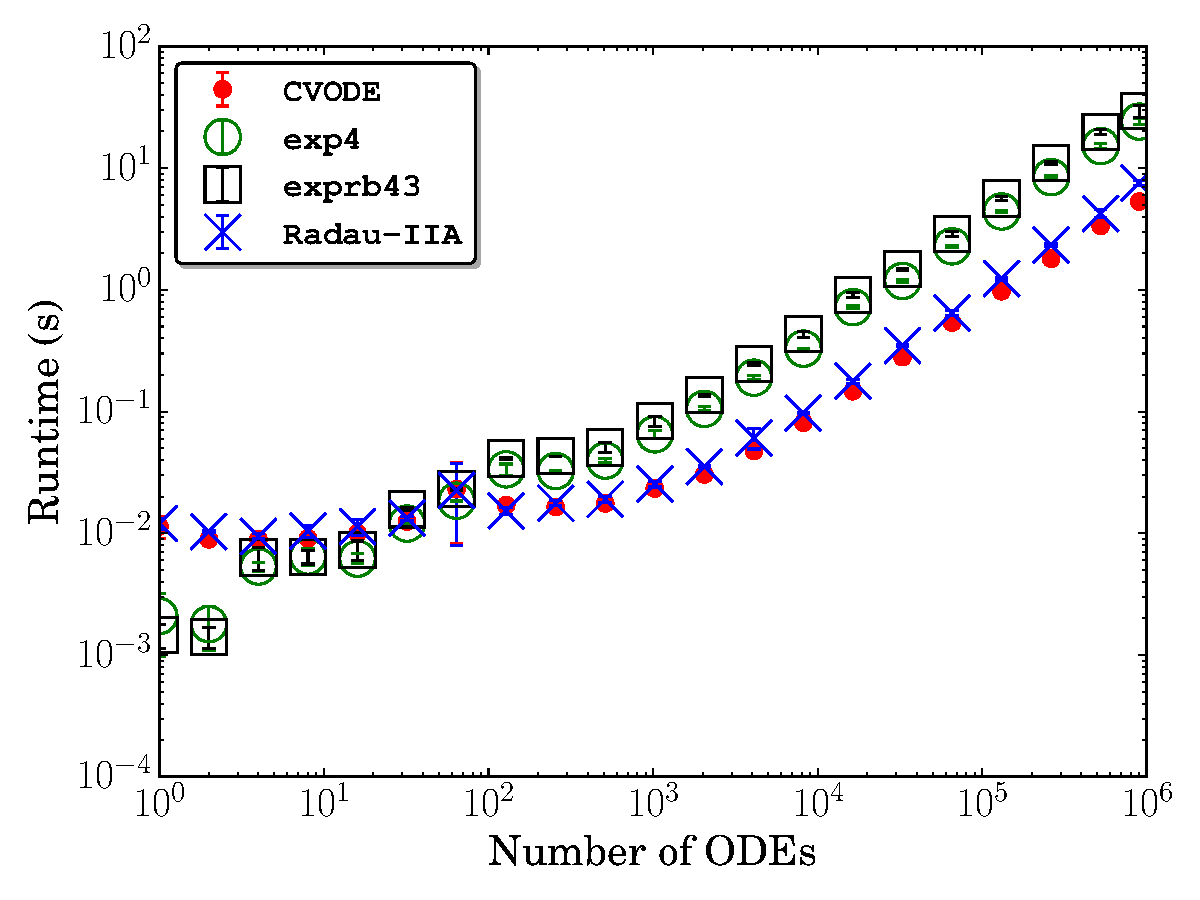
\includegraphics[width=\linewidth]{H2_1e-04_cpu_nonorm.pdf}
      \caption{CPU performance for $\delta t = \SI{e-4}{\sec}$}
 
  \end{subfigure}\\
  \begin{subfigure}{0.49\textwidth}
      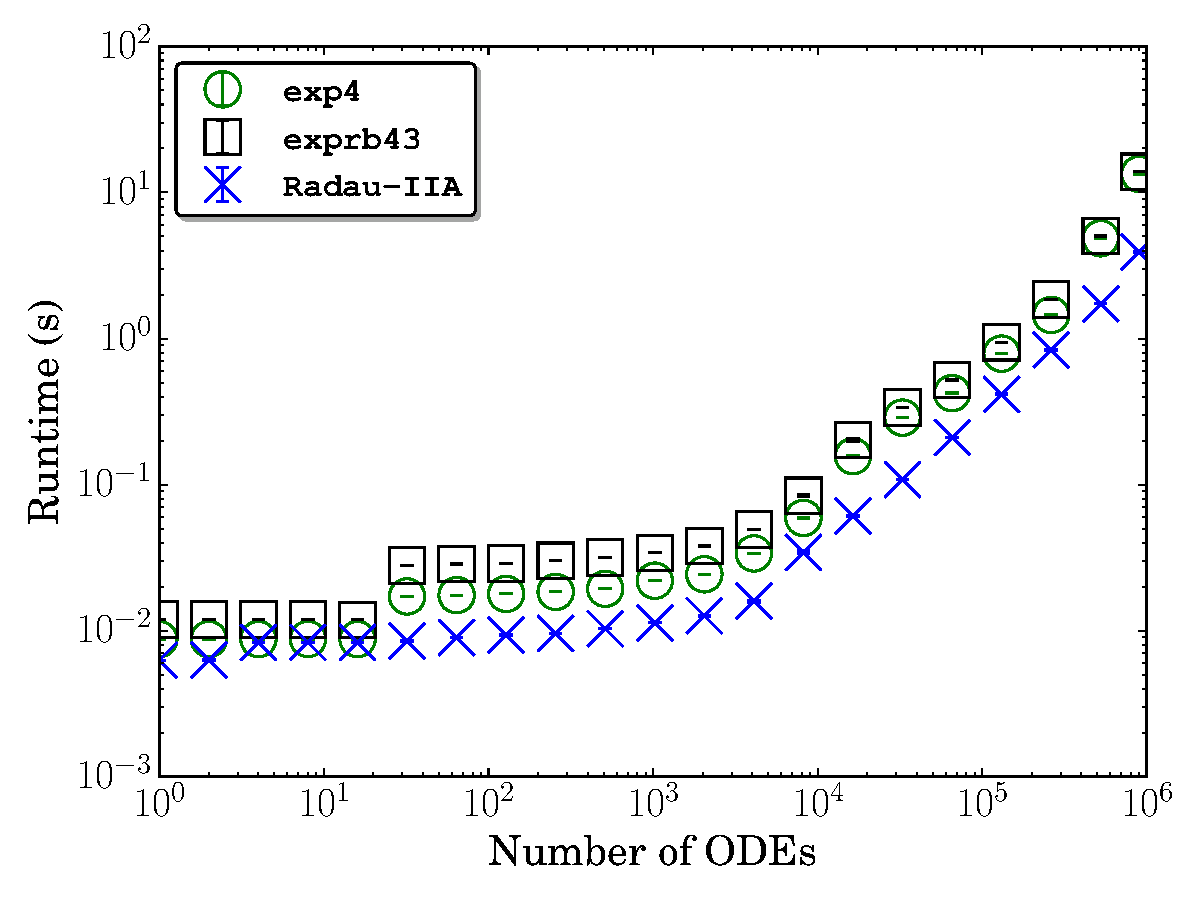
\includegraphics[width=\linewidth]{H2_1e-06_gpu_nonorm.pdf}
      \caption{GPU performance results for $\delta t = \SI{e-6}{\sec}$}
  \end{subfigure}
  %\hfill
  \begin{subfigure}{0.49\textwidth}
      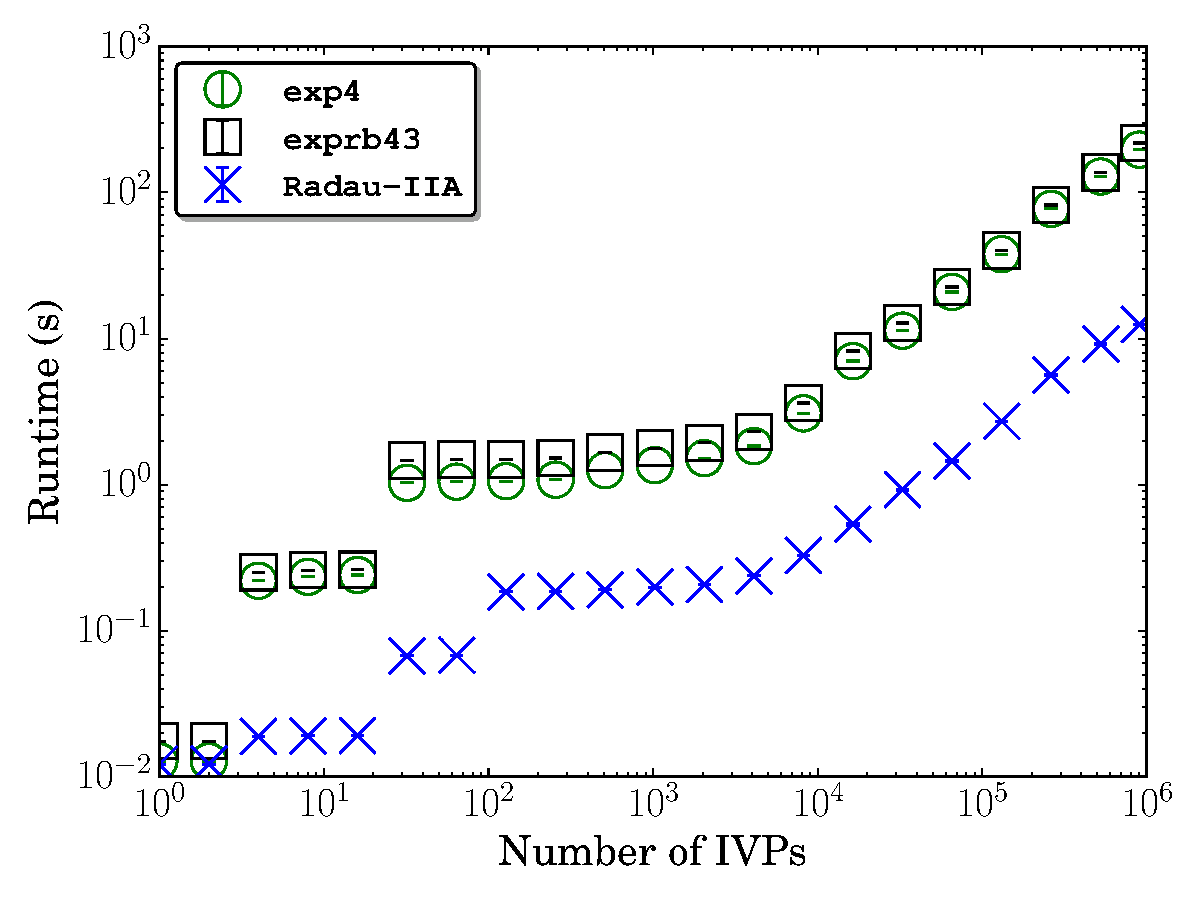
\includegraphics[width=\linewidth]{H2_1e-04_gpu_nonorm.pdf}
      \caption{GPU performance results for $\delta t = \SI{e-4}{\sec}$}
  \end{subfigure}
  \caption{Average (unnormalized) runtimes of the integrators on the CPU\slash GPU for the \ce{H2}\slash\ce{CO} model at two different global time-step sizes.}
\end{figure}

\begin{figure}[htb]
  \centering
  \begin{subfigure}{0.49\textwidth}
      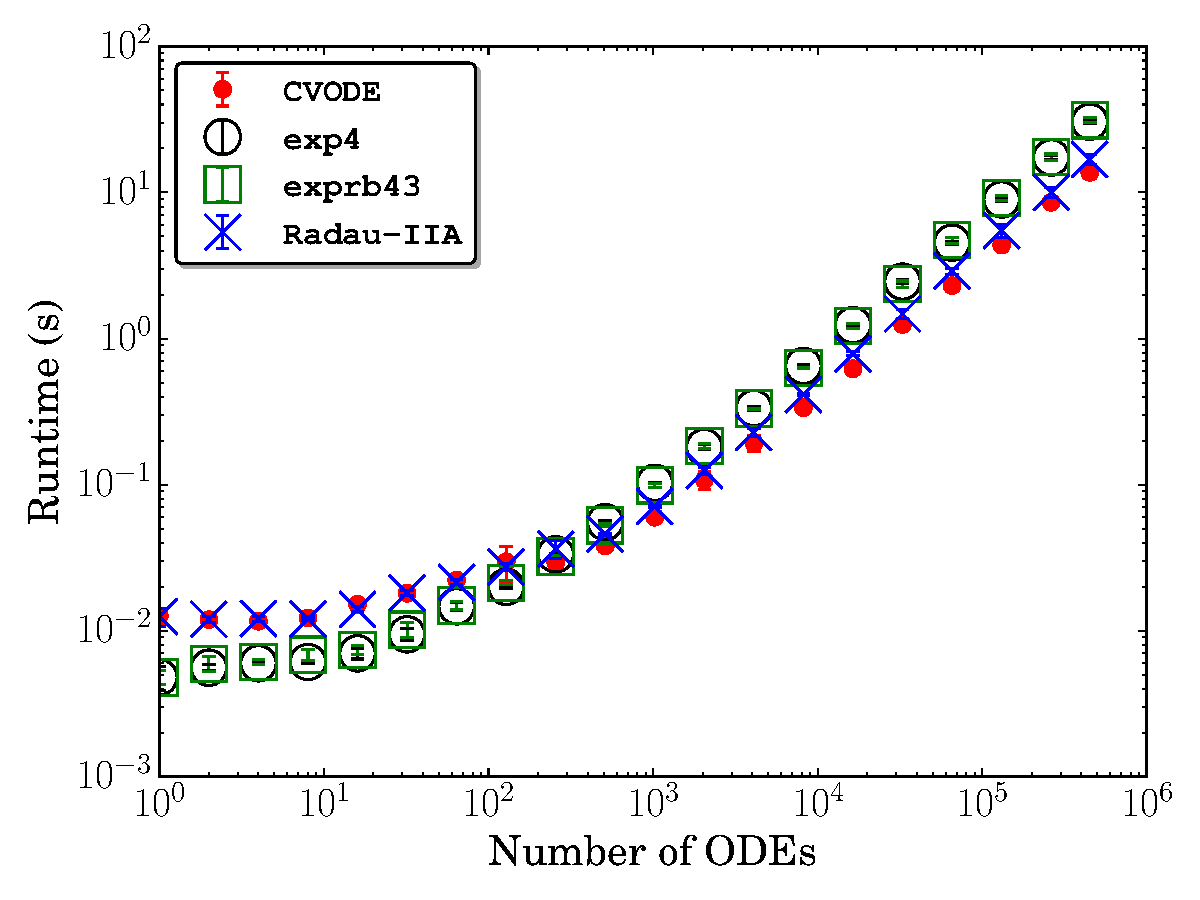
\includegraphics[width=\linewidth]{CH4_1e-06_cpu_nonorm.pdf}
      \caption{CPU performance for $\delta t = \SI{e-6}{\sec}$}
  \end{subfigure}
  %\hfill
  \begin{subfigure}{0.49\textwidth}
      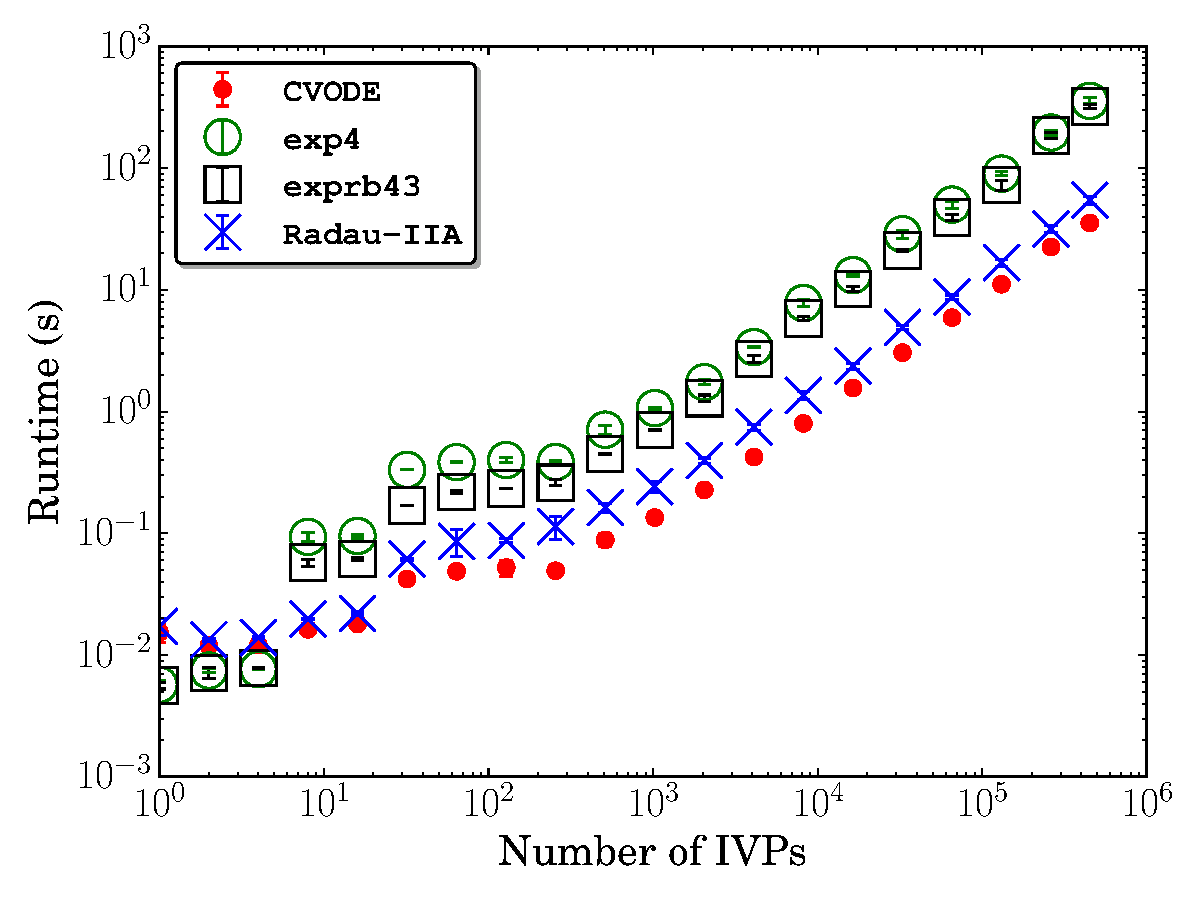
\includegraphics[width=\linewidth]{CH4_1e-04_cpu_nonorm.pdf}
      \caption{CPU performance for $\delta t = \SI{e-4}{\sec}$}
  \end{subfigure}\\
  \begin{subfigure}{0.49\textwidth}
      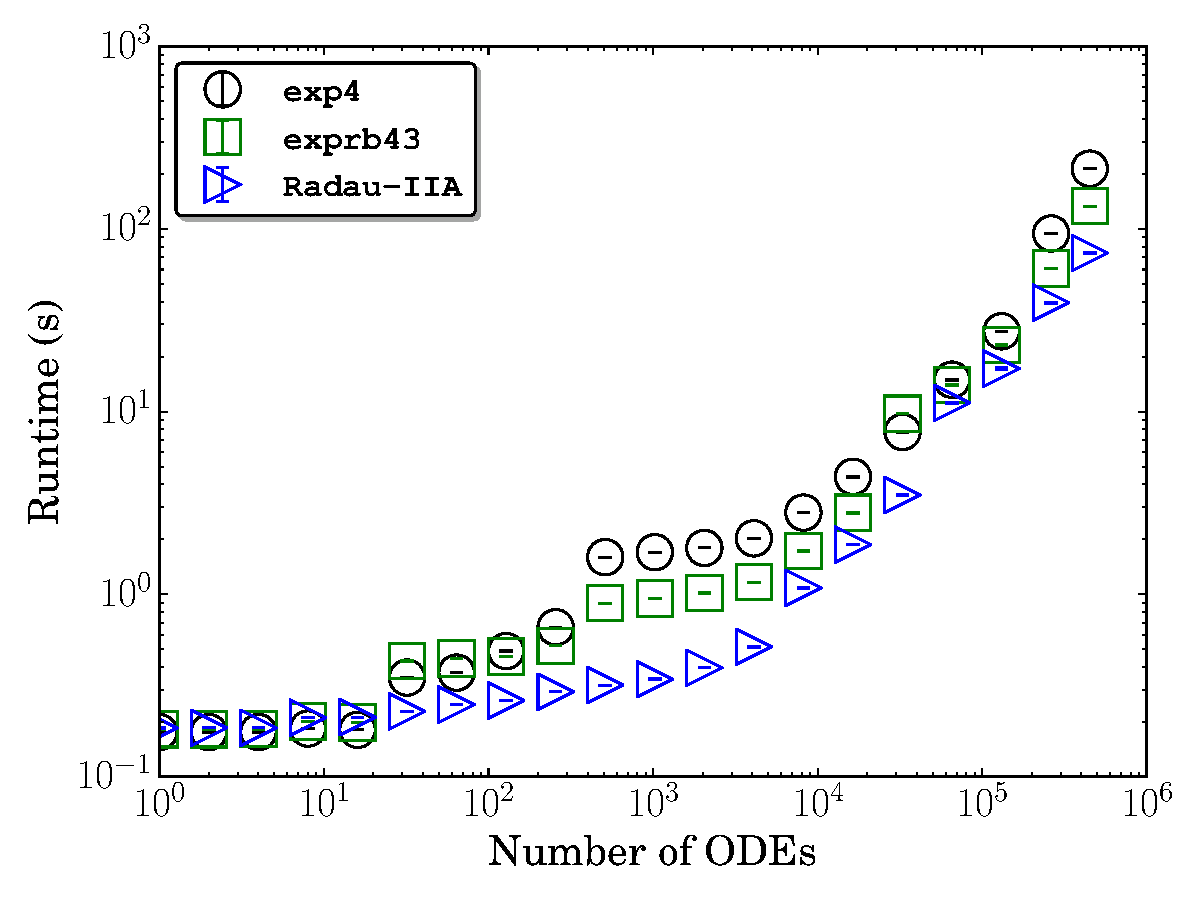
\includegraphics[width=\linewidth]{CH4_1e-06_gpu_nonorm.pdf}
      \caption{GPU performance results for $\delta t = \SI{e-6}{\sec}$}
  \end{subfigure}
  %\hfill
  \begin{subfigure}{0.49\textwidth}
      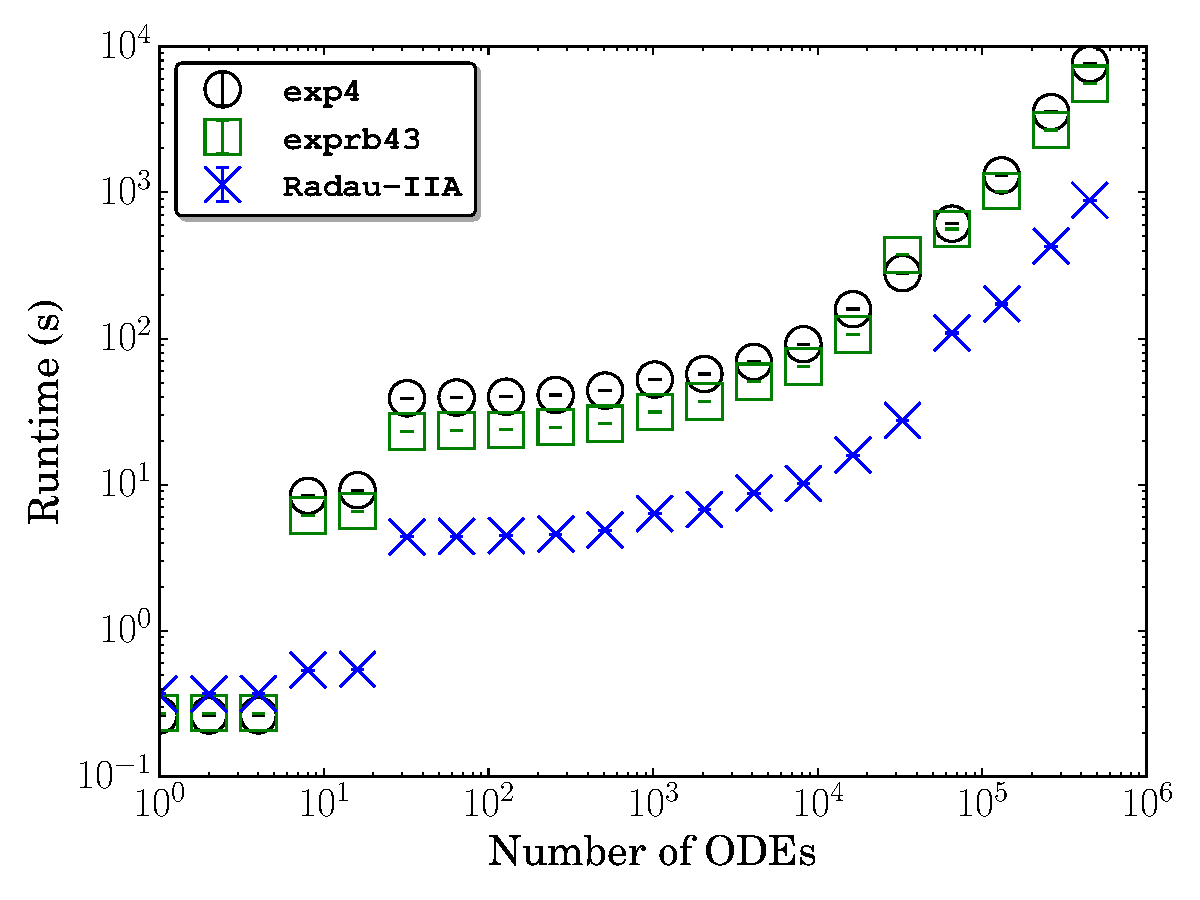
\includegraphics[width=\linewidth]{CH4_1e-04_gpu_nonorm.pdf}
      \caption{GPU performance results for $\delta t = \SI{e-4}{\sec}$}
  \end{subfigure}
  \caption{Average (unnormalized) runtimes of the integrators on the CPU\slash GPU for the GRI-Mech 3.0 model at two different global time-step sizes.}
\end{figure}

\clearpage

\bibliography{GPU-integrator-paper}
\bibliographystyle{elsarticle-num}

\end{document}
